\documentclass{article}

\usepackage{fontspec}
\usepackage{comment}
\usepackage{amsmath, mathtools}
\usepackage{fontspec,xgreek,polyglossia}
\usepackage{graphicx}
\usepackage{float}
\usepackage{hyperref}
\usepackage{url}
\usepackage{siunitx}
\usepackage{caption}
\usepackage{subfigure}
\usepackage{listings}

\renewcommand{\lstlistingname}{Έξοδος προγράμματος}

\hypersetup{
    colorlinks,
    citecolor=black,
    filecolor=black,
    linkcolor=black,
    urlcolor=black
}

\graphicspath{ {./images/} }
\defaultfontfeatures{Mapping=tex-text}
\setmainfont{Times New Roman}
\setdefaultlanguage[variant=modern]{greek}
\setotherlanguage{english}

\title{Ενσωματωμένο Σύστημα Αντί-Mπλοκαρίσματος Τροχών (ABS)}
\author{Σταυρόπουλος Σπυρίδων 1058691, Συμεωνίδης Θεόδωρος 1064870}
\date{Ακαδημαϊκό έτος 2020-21}
   
\begin{document}

\maketitle

\newpage

\tableofcontents

\newpage 

\section{Εισαγωγή}
 Ο σκοπός της παρούσας εργασίας είναι η μελέτη, ανάλυση και σχεδίαση ενός ενσωματωμένου συστήματος Αντί-μπλοκαρίσματος Τροχών (Anti-lock Braking System) ενός αυτοκινήτου. Πρόκειται για ένα σύστημα που αποτελείται από ηλεκτρονικά, μηχανικά και υδραυλικά μέρη. Έρχεται να βελτιώσει και να διασφαλίσει τη διαδικασία της πέδησης του οχήματος. Προσφέρει περισσότερο έλεγχο του τιμονιού στον οδηγό κατά τη διαδικασία και συνήθως μειώνει το χρόνο πέδησης. Πρόκειται για ένα αυτοματοποιημένο σύστημα υλοποίησης των τεχνικών threshold braking και cadence braking που χρησιμοποιείται από οδηγούς στο μηχανοκίνητο αθλητισμό.

\subsection{Ιστορικά στοιχεία}
Η βασική ιδέα πίσω από το ABS πρωτοεμφανίστηκε το 1908 σε ένα σύστημα για τρένα. Αργότερα, το 1920 η ιδέα αυτή άρχισε να ενσωματώνεται σε συστήματα πέδησης αεροπλάνων αυξάνοντας σημαντικά τον έλεγχο του πιλότου του κατά την προσγείωση. Αξίζει να σημειωθεί ότι η καταπόνηση που αντιμετωπίζουν τα ελαστικά των αεροσκαφών είναι πολύ μεγαλύτερης κλίμακας σε σχέση με αυτής των επιβατικών αυτοκινήτων. Με το ABS μειώθηκαν περιστατικά που ο πιλότος φρέναρε απότομα με αποτέλεσμα να εκραγούν τα ελαστικά του αεροπλάνου και αύξησε τον έλεγχο του πιλότου. Η τεχνολογία βρισκόταν σε πρωταρχικά στάδια, αλλά συνέχισε να βελτιώνεται και να ενσωματώνεται σε όλο και περισσότερα αεροσκάφη τη δεκαετία του ’50, και το ’58 εφαρμόστηκε πειραματικά σε μια μοτοσυκλέτα. Ύστερα βρήκε μεμονωμένη εφαρμογή σε κάποια αυτοκίνητα. Αξιοσημείωτο ήταν κατά το τέλος της δεκαετίας του ’60 που υλοποιήθηκε το πρώτο ηλεκτρονικό ABS (πιο πριν χρησιμοποιούνταν ένα σύστημα με σφονδύλους, που δεν έχει σχέση με το σύγχρονο ABS και δεν θα το μελετήσουμε) και βρήκε εφαρμογή σε ένα από τα γρηγορότερα επιβατικά αεροσκάφη (μέχρι και σήμερα) το Concorde. Από το 1970 και μετά εφαρμόζεται σε αυτοκίνητα. Έτσι είναι υποχρεωτικό πλέον σε όλα τα αμάξια που πωλούνται μετά το 2004 στην Ευρώπη και μετά το 2013 στις Η.Π.Α. .

\section{Περιγραφή προβλήματος}
Κατά την πέδηση ενός αυτοκινήτου ένας ή περισσότεροι τροχοί μπορεί να μπλοκάρουν με συνέπεια να χαθεί ο έλεγχος του τιμονιού, η απόσταση πέδησης να αυξηθεί και η φθορά των ελαστικών να είναι ανομοιόμορφη. Για να κατανοήσουμε το πρόβλημα πρέπει να καταλάβουμε το μηχανισμό και τους φυσικούς νόμους που διέπουν το φρενάρισμα ενός αμαξιού χωρίς ABS. Στη συνέχεια θα περιγράψουμε μέσω ενός απλού μοντέλου τη διαδικασία αυτής. Υπό κανονικές συνθήκες, το αμάξι κινείται χωρίς να ολισθαίνει, τότε ισχύει $V=\omega\times R$. Κατά την πέδηση, ο οδηγός πιέζοντας το πεντάλ του φρένου δημιουργεί μια πίεση στο υγρό των φρένων η οποία μέσω ενός κλειστού κυκλώματος ροής μεταφέρεται στα τακάκια τα οποία πιέζουν το δισκόφρενο που είναι τοποθετημένο στη ρόδα, αυτό προκαλεί στη ρόδα γωνιακή επιβράδυνση και υπό συνθήκες απότομου σταματήματος έχουμε $V >\omega\times R$. Τότε εμφανίζεται τριβή ολίσθησης στο σημείο επαφής του τροχού με το έδαφος με κατεύθυνση αντίθετη του $V$ η οποία τείνει να εξαλείψει την ανισορροπία που υπάρχει μεταξύ την απόστασης που διανύεται λόγω $V$ και της απόστασης που διανύεται λόγω $\omega$. Αυτή η δύναμη αυξάνει την απόσταση που διανύεται λόγω γωνιακής ταχύτητας, η οποία για ένα χρονικό διάστημα $\Delta t$ είναι $\Delta x_v = \Delta V \cdot \Delta t$ και μειώνει την απόσταση που διανύεται λόγω μεταφορικής ταχύτητας, και αντίστοιχα είναι $\Delta x_\omega = \Delta \omega \cdot \Delta t \cdot R$. Ωστόσο κατά τη διαδικασία αυτή χάνεται ενέργεια και έτσι αν επαναληφθεί η διαδικασία αυτή αρκετές φορές επιβραδύνεται το αμάξι μέχρι να σταματήσει. Η τριβή μεταξύ της ρόδας και του εδάφους είναι αυτή που προκαλεί την επιβράδυνση και όχι η δύναμη που ασκούν τα τακάκια στη ρόδα. Σε απότομα φρεναρίσματα χωρίς ABS αυτοκινήτων δεν είναι σπάνιο, να έχει ακινητοποιηθεί η ρόδα ως προς το αμάξι (τακάκια), ωστόσο να μην έχει ακινητοποιηθεί ως προς το έδαφος με αποτέλεσμα το όχημα να ολισθαίνει. 

Όταν το όχημα ολισθαίνει το ποσοστό ολίσθησης δίνεται από τον τύπο $S=\frac{V-\omega\times R}{V}$ και έχει εκτιμηθεί ότι ο μέγιστος συντελεστής τριβής $\mu$ ανάμεσα στο τροχό και το οδόστρωμα αναπτύσσεται όταν $S=\kappa\epsilon[0.05,0.2]$ όπως φαίνεται στο Σχήμα \ref{fig:slip-friction-diagram}. To $\kappa$ μεταβάλλεται ανάλογα με τον τύπο του οδοστρώματος και του ελαστικού.

\begin{figure}[H]
    \begin{center}
    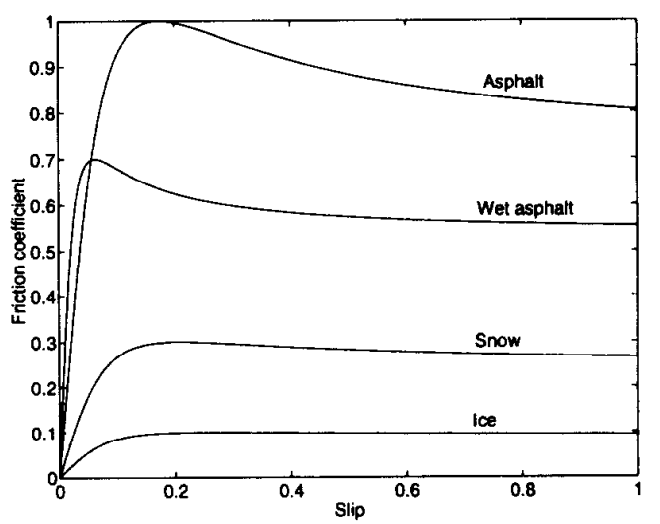
\includegraphics[scale=0.4]{images/slip-friction-diagram.png}
    \end{center}
    \caption{Γραφική παράσταση $\mu$-$S$ σε διαφορετικά είδη επιφανειών \cite{10.1016/S0005-1098(97)00003-4}}
    \label{fig:slip-friction-diagram}
\end{figure}

\section{Λειτουργικές απαιτήσεις χρήστη}
Το σύστημα απαιτεί αλληλεπίδραση με το χρήστη καθώς η ενεργοποίηση/απενεργο\-ποίηση του εξαρτάται από το πόσο πατάει η χρήστης το φρένο. Υπενθυμίζεται πως θέλουμε να ενεργοποιείται μόνος σε καταστάσεις πολύ απότομης πέδησης καθώς προκαλεί ολίσθηση που φθείρει τα ελαστικά. Θα πρέπει να αποκρίνεται στον ελάχιστο δυνατό χρόνο καθότι συνήθως ενεργοποιείται σε συνθήκες που μπορούν να οδηγήσουν σε κάποιο ατύχημα. Επίσης, χρειάζεται να είναι αξιόπιστο, να μπορεί να λειτουργεί σε εύρος συνθηκών και να είναι προβλέψιμο. Τέλος, θα πρέπει να προσφέρει κατά το δυνατό περισσότερο έλεγχο του τιμονιού στο φρενάρισμα και ελάττωση του χρόνου πέδησης.

\newpage

\section{Προδιαγραφές συστήματος}
Το σύστημα μας απαιτεί:
\begin{itemize}

\item Μεγάλη αξιοπιστία σε μεγάλο εύρος συνθηκών οδοστρώματος, π.χ. βρεγμένο, παγωμένο και ξηρό. Ανθεκτικότητα στις υψηλές θερμοκρασίες που αναπτύσσονται αλλά και στο περιβάλλον έντονου ηλεκτρομαγνητικού θορύβου στο οποίο καλείται να λειτουργήσει. Θα θέλαμε δηλαδή τα συστατικά των υποσυστημάτων να είναι συμβατά με πρότυπα της βιομηχανίας αυτοκινήτων, όπως το AEC-Q100.
\item Επεξεργαστές υψηλής συχνότητας λειτουργίας και δειγματοληψίας γιατί πρόκειται για hard real-time σύστημα.
\item {Δυνατότητα λήψης αποφάσεων τουλάχιστον 10 φορές το δευτερόλεπτο για κάθε ρόδα ξεχωριστά δηλαδή δυνατότητα εκτέλεσης τουλάχιστον 10 κύκλων αυξομείωσης της πίεσης του συστήματος το δευτερόλεπτο.}\label{tenTimesPerSec}
\item Δυνατότητα για κάθε τροχό να μπορούμε ξεχωριστά να αποκόπτουμε/ελευθερώνουμε την πίεση των υδραυλικών των φρένων της από/προς το κυρίως δοχείο υγρού φρένων \footnote{Αυτό δεν απαιτεί τόσο αυστηρή απαίτηση. Επειδή πολλά αυτοκίνητα δεν διαθέτουν φρένα και στους 4 τροχούς, υπάρχουν αρχιτεκτονικές ABS που αντιμετωπίζουν τους 2 τροχούς ως ξεχωριστό κύκλωμα και τους άλλους 2 ως ενιαίο. Αυτό αποτελεί μια απλούστευση στο πρόβλημα μας. }.
\item Σχετικά εύκολη τοποθέτηση και συντήρηση.
\end{itemize}

\section{Προσέγγιση λογισμικού}
Ο μικροελεγκτής, όταν πατηθεί απότομα το πεντάλ του φρένου, ελέγχει για ασυνήθιστες τιμές τους αισθητήρες. Αν η γωνιακή ταχύτητα κάποιου τροχού παρουσιάσει ανωμαλία που φανερώνει ολίσθηση με μη επιθυμητό $S>\kappa$ όπου $\kappa$ είναι ένα όριο που καθορίζει ο αλγόριθμος, τότε πρέπει να μειώσουμε τη δύναμη που ασκούν τα τακάκια στο τροχό ώστε να αποκτήσει ταχύτητα. Για να το πετύχουμε αυτό κλείνουμε την βαλβίδα εισόδου ώστε να αποτρέψει περαιτέρω μεταφορά πίεσης από τον πεντάλ του φρένου στο δισκόφρενο. Αν ο τροχός συνεχίσει να ολισθαίνει, δίνουμε σήμα στον οδηγό της βαλβίδας εξόδου να ανοίξει και στον οδηγό της αντλίας ώστε να ελαττωθεί η πίεση που ασκείται στο τροχό η οποία θα έχει ως συνέπεια αυτός να αρχίσει να ολισθαίνει λιγότερο. Ελέγχουμε τον τροχό μέσω του αισθητήρα γωνιακής ταχύτητας σε περίπτωση που έχουμε μη επιθυμητό $S<\kappa$. Τότε πρέπει να δώσουμε σήμα στον οδηγό να ανοίξει τη βαλβίδα εισόδου ώστε να φτάσει πίεση στα δισκόφρενα και να αυξηθεί η ολίσθηση στα επιθυμητά όρια. Επαναλαμβάνουμε την παραπάνω διαδικασία όσο ο οδηγός πατάει το πεντάλ του φρένου.

\begin{figure}[H]
    \begin{center}
    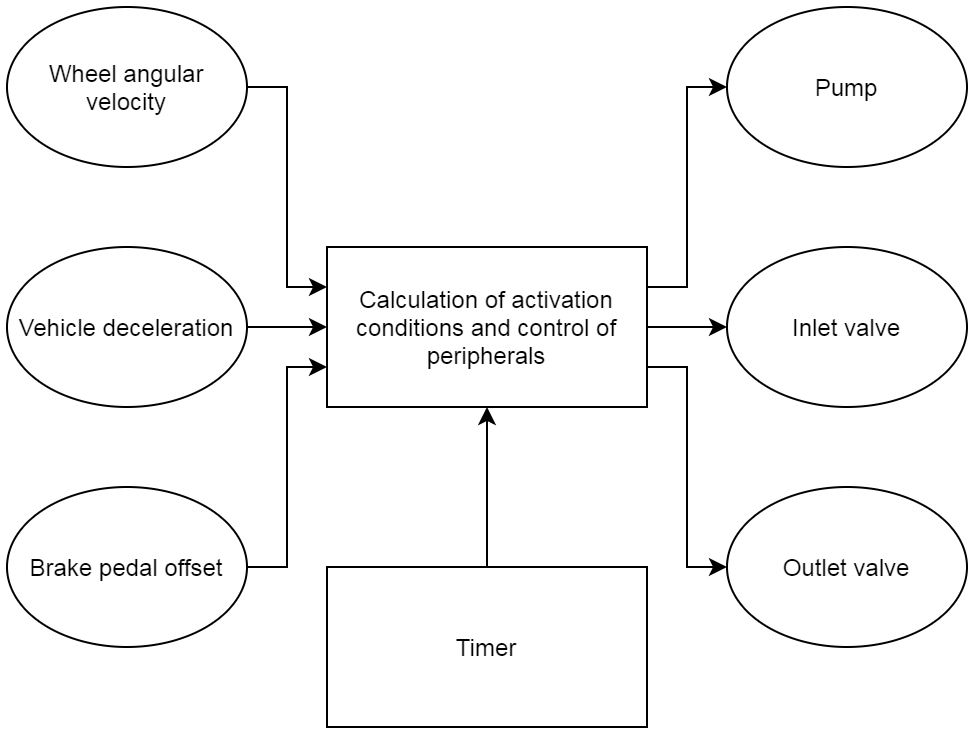
\includegraphics[scale=0.30]{images/software-architecture-preview.png}
    \end{center}
    \caption{Αρχιτεκτονική λογισμικού του συστήματος.}
    \label{fig:software-architecture-preview}
\end{figure}


\section{Προσέγγιση υλικού}
Το σύστημα μας αποτελείται από 3 αισθητήρες (είσοδοι) και 3 actuators (έξοδοι). Για την επικοινωνία με αυτά τα μέρη του συστήματος θα χρησιμοποιήσουμε οδηγούς. Όλα αυτά τα μέρη θα συνδέονται σε έναν δίαυλο όπως φαίνεται στο Σχήμα \ref{fig:hardware-architecture-preview}.
Για τον αναγνώστη που ενδιαφέρεται να αποκτήσει μια πλήρη εικόνα του συστήματος παραθέτουμε και τα υδραυλικά/ηλεκτρικά μέρη στο Σχήμα \ref{fig:hydraulic-mechanical-system-preview}.

\begin{figure}[H]
    \begin{center}
    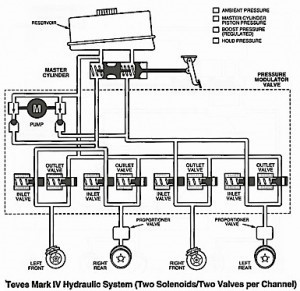
\includegraphics[scale=0.6]{images/hydraulic-mechanical-system-overview.jpg}
    \end{center}
    \caption{Μηχανικά και υδραυλικά μέρη μιας υλοποίησης ABS.}
    \label{fig:hydraulic-mechanical-system-preview}
\end{figure}

\begin{figure}[H]
    \begin{center}
    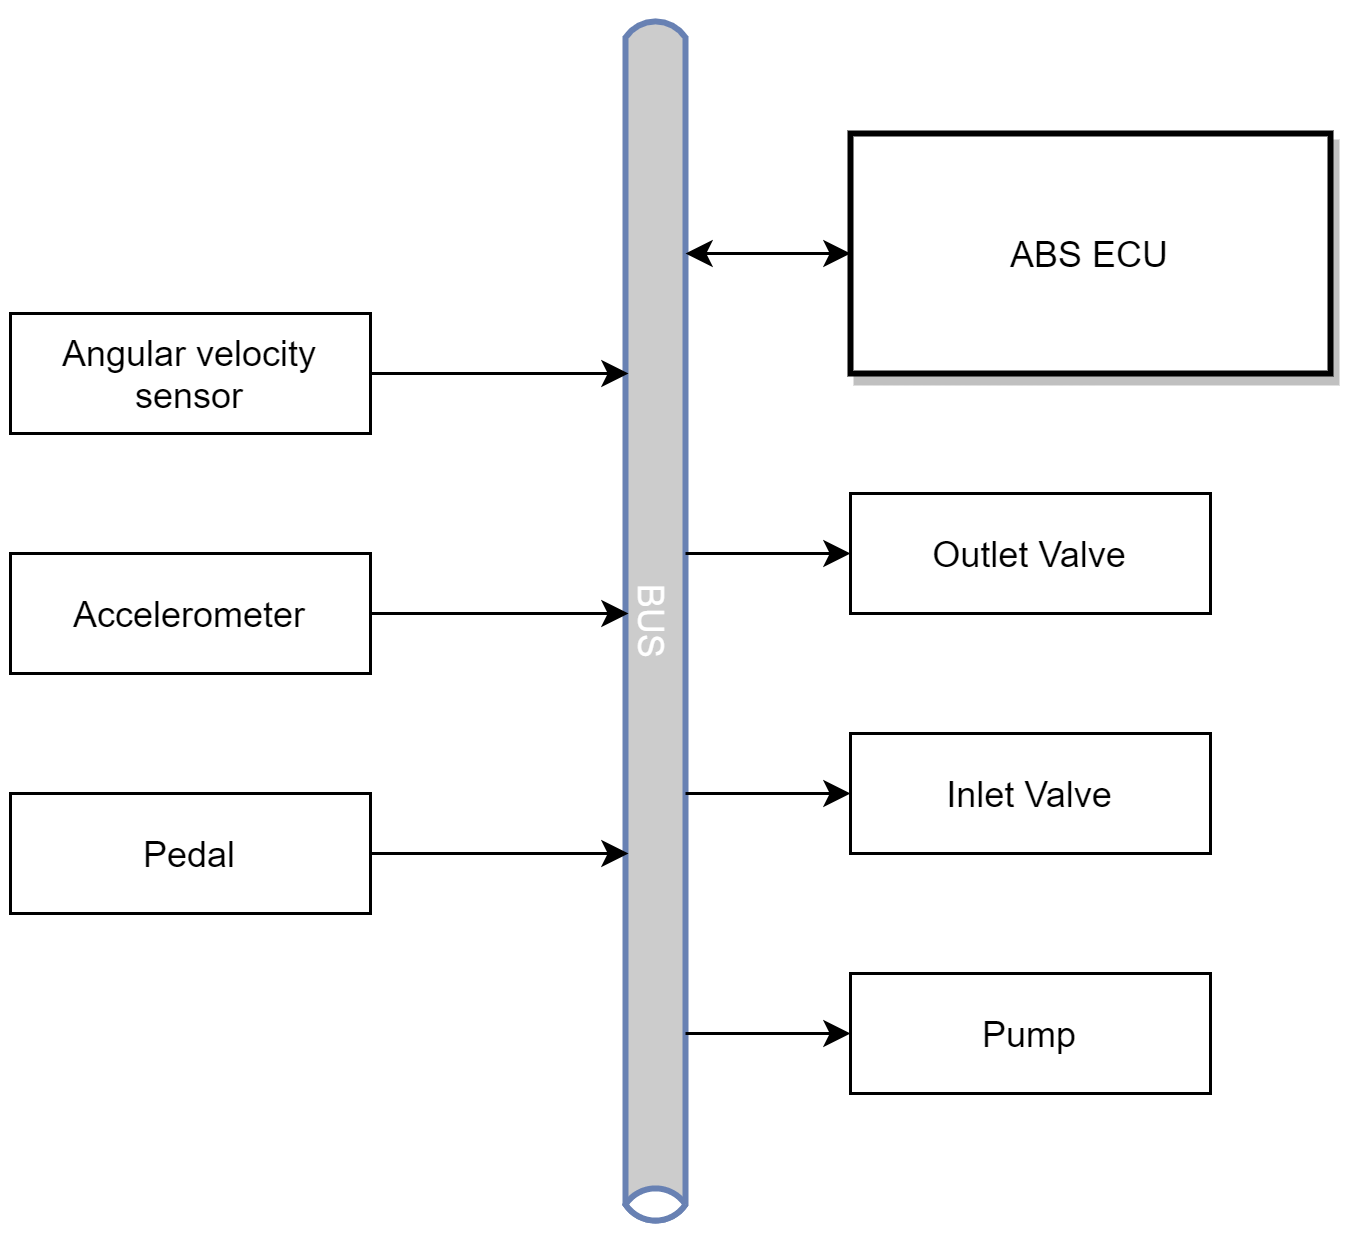
\includegraphics[scale=0.15]{images/hardware-architecture-preview.png}
    \end{center}
    \caption{Προσεγγιστική αρχιτεκτονική υλικού ABS συστήματος.}
    \label{fig:hardware-architecture-preview}
\end{figure}


\section{Αλγόριθμος}
Για τη σχεδίαση του συστήματος μας κρίθηκε απαραίτητη η επιλογή ενός αλγορίθμου, ο οποίος θα καθορίζει πότε και κατά πόσο θα πρέπει να αυξάνεται/μειώνεται η πέδηση των τροχών και κατά συνέπεια πότε θα ενεργοποιούνται/απενεργοποιούνται τα επιμέρους υποσυστήματα που το κάνουν πράξη. Οι σχεδιαστικοί περιορισμοί που εισάγει η επιλογή ενός αλγορίθμου ABS είναι το πλήθος των εισόδων που απαιτεί για την λήψη αποφάσεων. Αυτό επηρεάζει με ποια υποσυστήματα αισθητήρων θα πρέπει να διασυνδέεται το Κεντρικό ABS ECU. Οι αλγόριθμοι για ABS αποτελούν ένα βαθιά μελετημένο πρόβλημα στη βιβλιογραφία της θεωρίας ελέγχου λόγω των μαθηματικών ιδιομορφιών του προβλήματος και οι περισσότεροι αλγόριθμοι που έχουν προταθεί είναι ιδιαίτερα πολύπλοκοι. Στα πλαίσια της παρούσας εργασίας αποφασίσαμε να χρησιμοποιήσουμε έναν από τους πιο απλούς που ικανοποιούν τις ανάγκες του συστήματος μας και προτάθηκε από τον G. F. Mauer \cite{481947}. Στην παρούσα φάση δεν θα ασχοληθούμε με τη ανάλυση του αλγορίθμου. Αρκούμαστε στο να γνωρίζουμε ότι ο αλγόριθμος απαιτεί αισθητήρες γωνιακής ταχύτητας στους τροχούς, επιταχυνσιόμετρο στο όχημα \footnote{Ο αλγόριθμος χρησιμοποιεί την επιτάχυνση για να υπολογίσει την ταχύτητα του οχήματος μέσω της ολοκλήρωσης της συνάρτησης. Χρειαζόμαστε την επιτάχυνση μόνο στη διεύθυνση του $Χ$ άξονα που είναι παράλληλος στον άξονα μετάδοσης του οχήματος } και μνήμη ώστε να αποθηκεύει αποτελέσματα από τις προηγούμενες μετρήσεις. Σημαντική λεπτομέρεια είναι πως ο αλγόριθμος αυτός είναι ικανός στο προβλέπει on-line το τύπο του οδοστρώματος στο οποίο συμβαίνει η πέδηση και να προσπαθεί να επιτύχει κατάλληλο $\kappa$ αντίστοιχα. Τέλος, ένας αλγόριθμος εισάγει και περιορισμούς ως προς τους υπολογιστικούς πόρους (επεξεργαστική ισχύ, μνήμη, ταχύτητα επικοινωνίας), αυτός που επιλέξαμε παρότι εκτελεί σχετικά λίγους υπολογισμούς ίσως να χρειαστεί έναν εξειδικευμένο συν-επεξεργαστή μαθηματικών υπολογισμών για επιτάχυνση των υπολογισμών που απαιτούν κινητή υποδιαστολή αν επιλεγεί η υλοποίηση του σε λογισμικό.

\section{Αρχιτεκτονική συστήματος}
Στο Σχήμα \ref{fig:system-architecture-overview} περιγράφεται με StateChart \cite{10.1016/0167-6423(87)90035-9} η αφ'υψηλού  αρχιτεκτονική της συμπεριφοράς του συστήματος στο Σχήμα \ref{fig:system-architecture-detailed} φαίνεται η λεπτομερής αρχιτεκτονική της συμπεριφοράς του συστήματος.
\par
Η φύση του συστήματος δεν αφήνει πολλά περιθώρια όσον αφορά την αρχιτεκτονική του υλικού και του λογισμικού του, δηλαδή το τι θα υλοποιηθεί σε υλικό και τι σε λογισμικό αλλά και το πού θα γίνουν αυτά. Οι κύριοι περιορισμοί που θα καθορίσουν την αρχιτεκτονική του συστήματος τίθενται από τις προδιαγραφές του και είναι ο χρόνος αντίδρασης, η αξιοπιστία και το περιβάλλον έντονου θορύβου μέσα στο οποίο καλείται να λειτουργήσει το σύστημα.

\begin{figure}[h]
    \begin{center}
    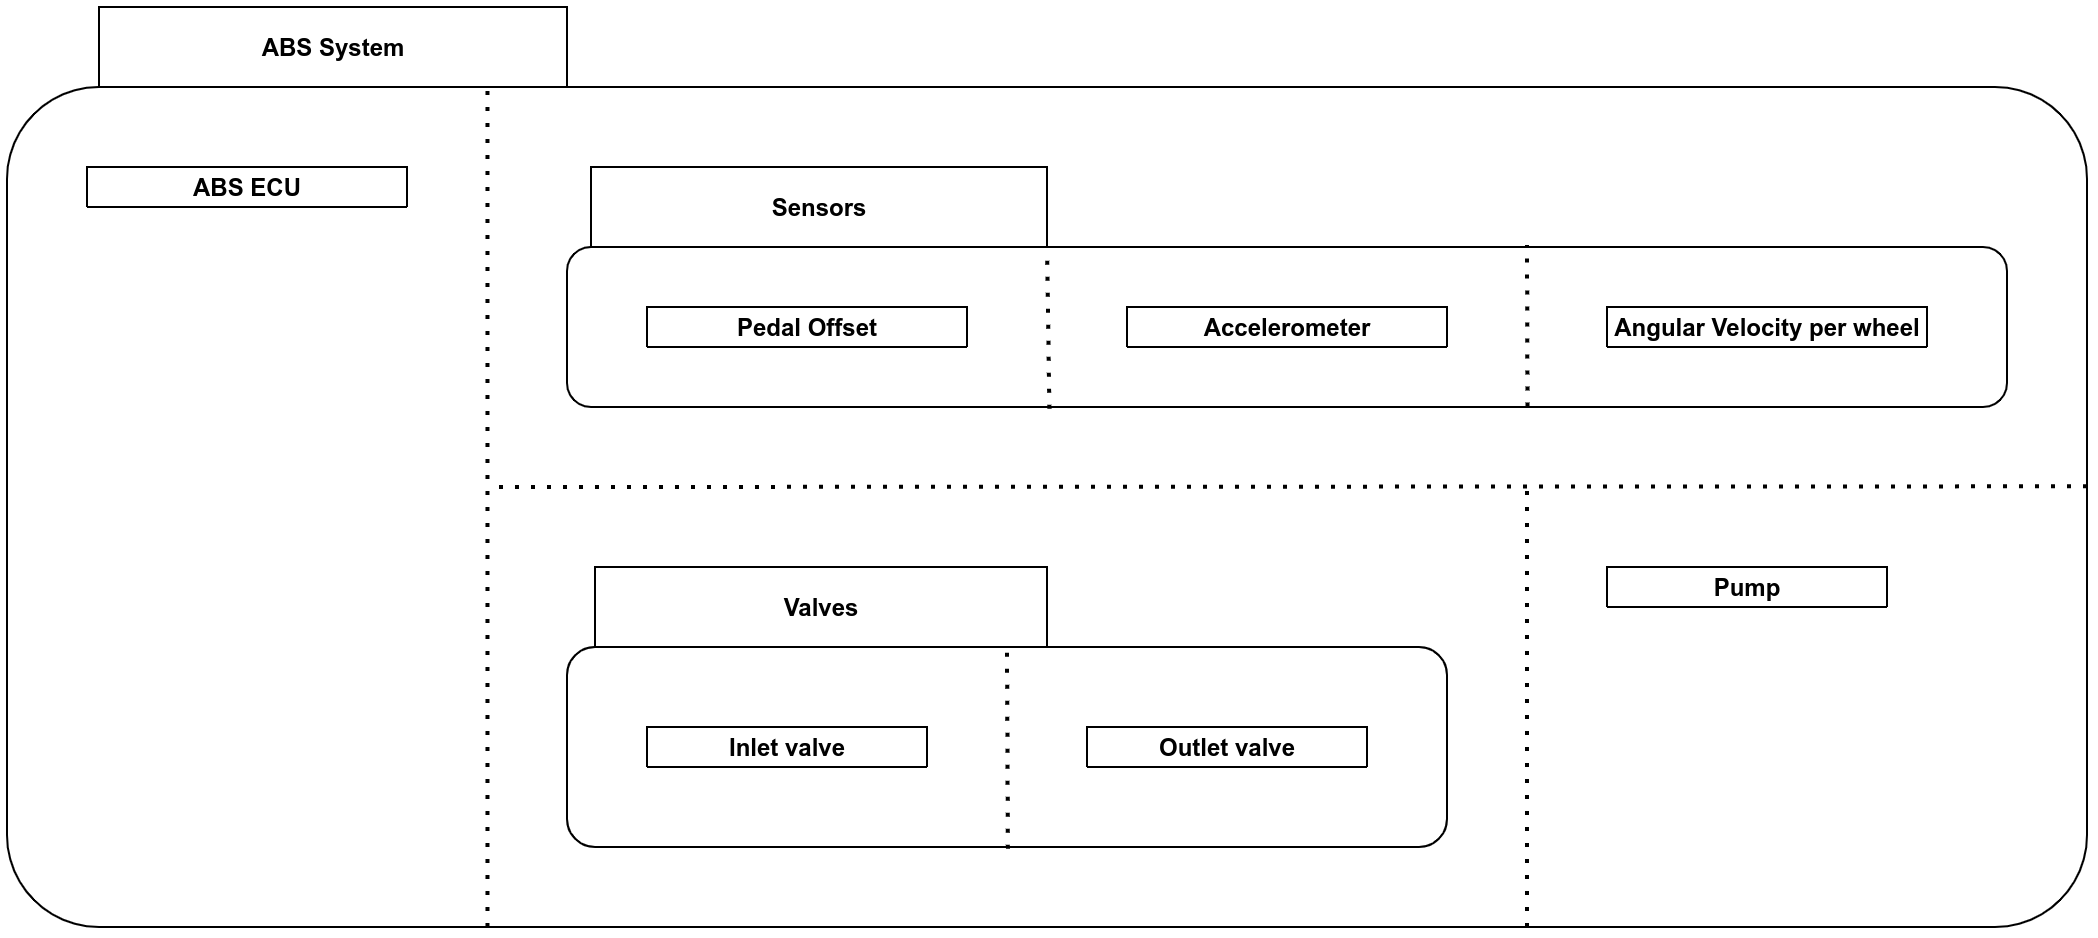
\includegraphics[scale=0.15]{images/system-architecture-overview.png}
    \end{center}
    \caption{Αρχιτεκτονική ABS συστήματος με StateChart.}
    \label{fig:system-architecture-overview}
\end{figure}

\begin{figure}[Η]
    \makebox[\textwidth][c]{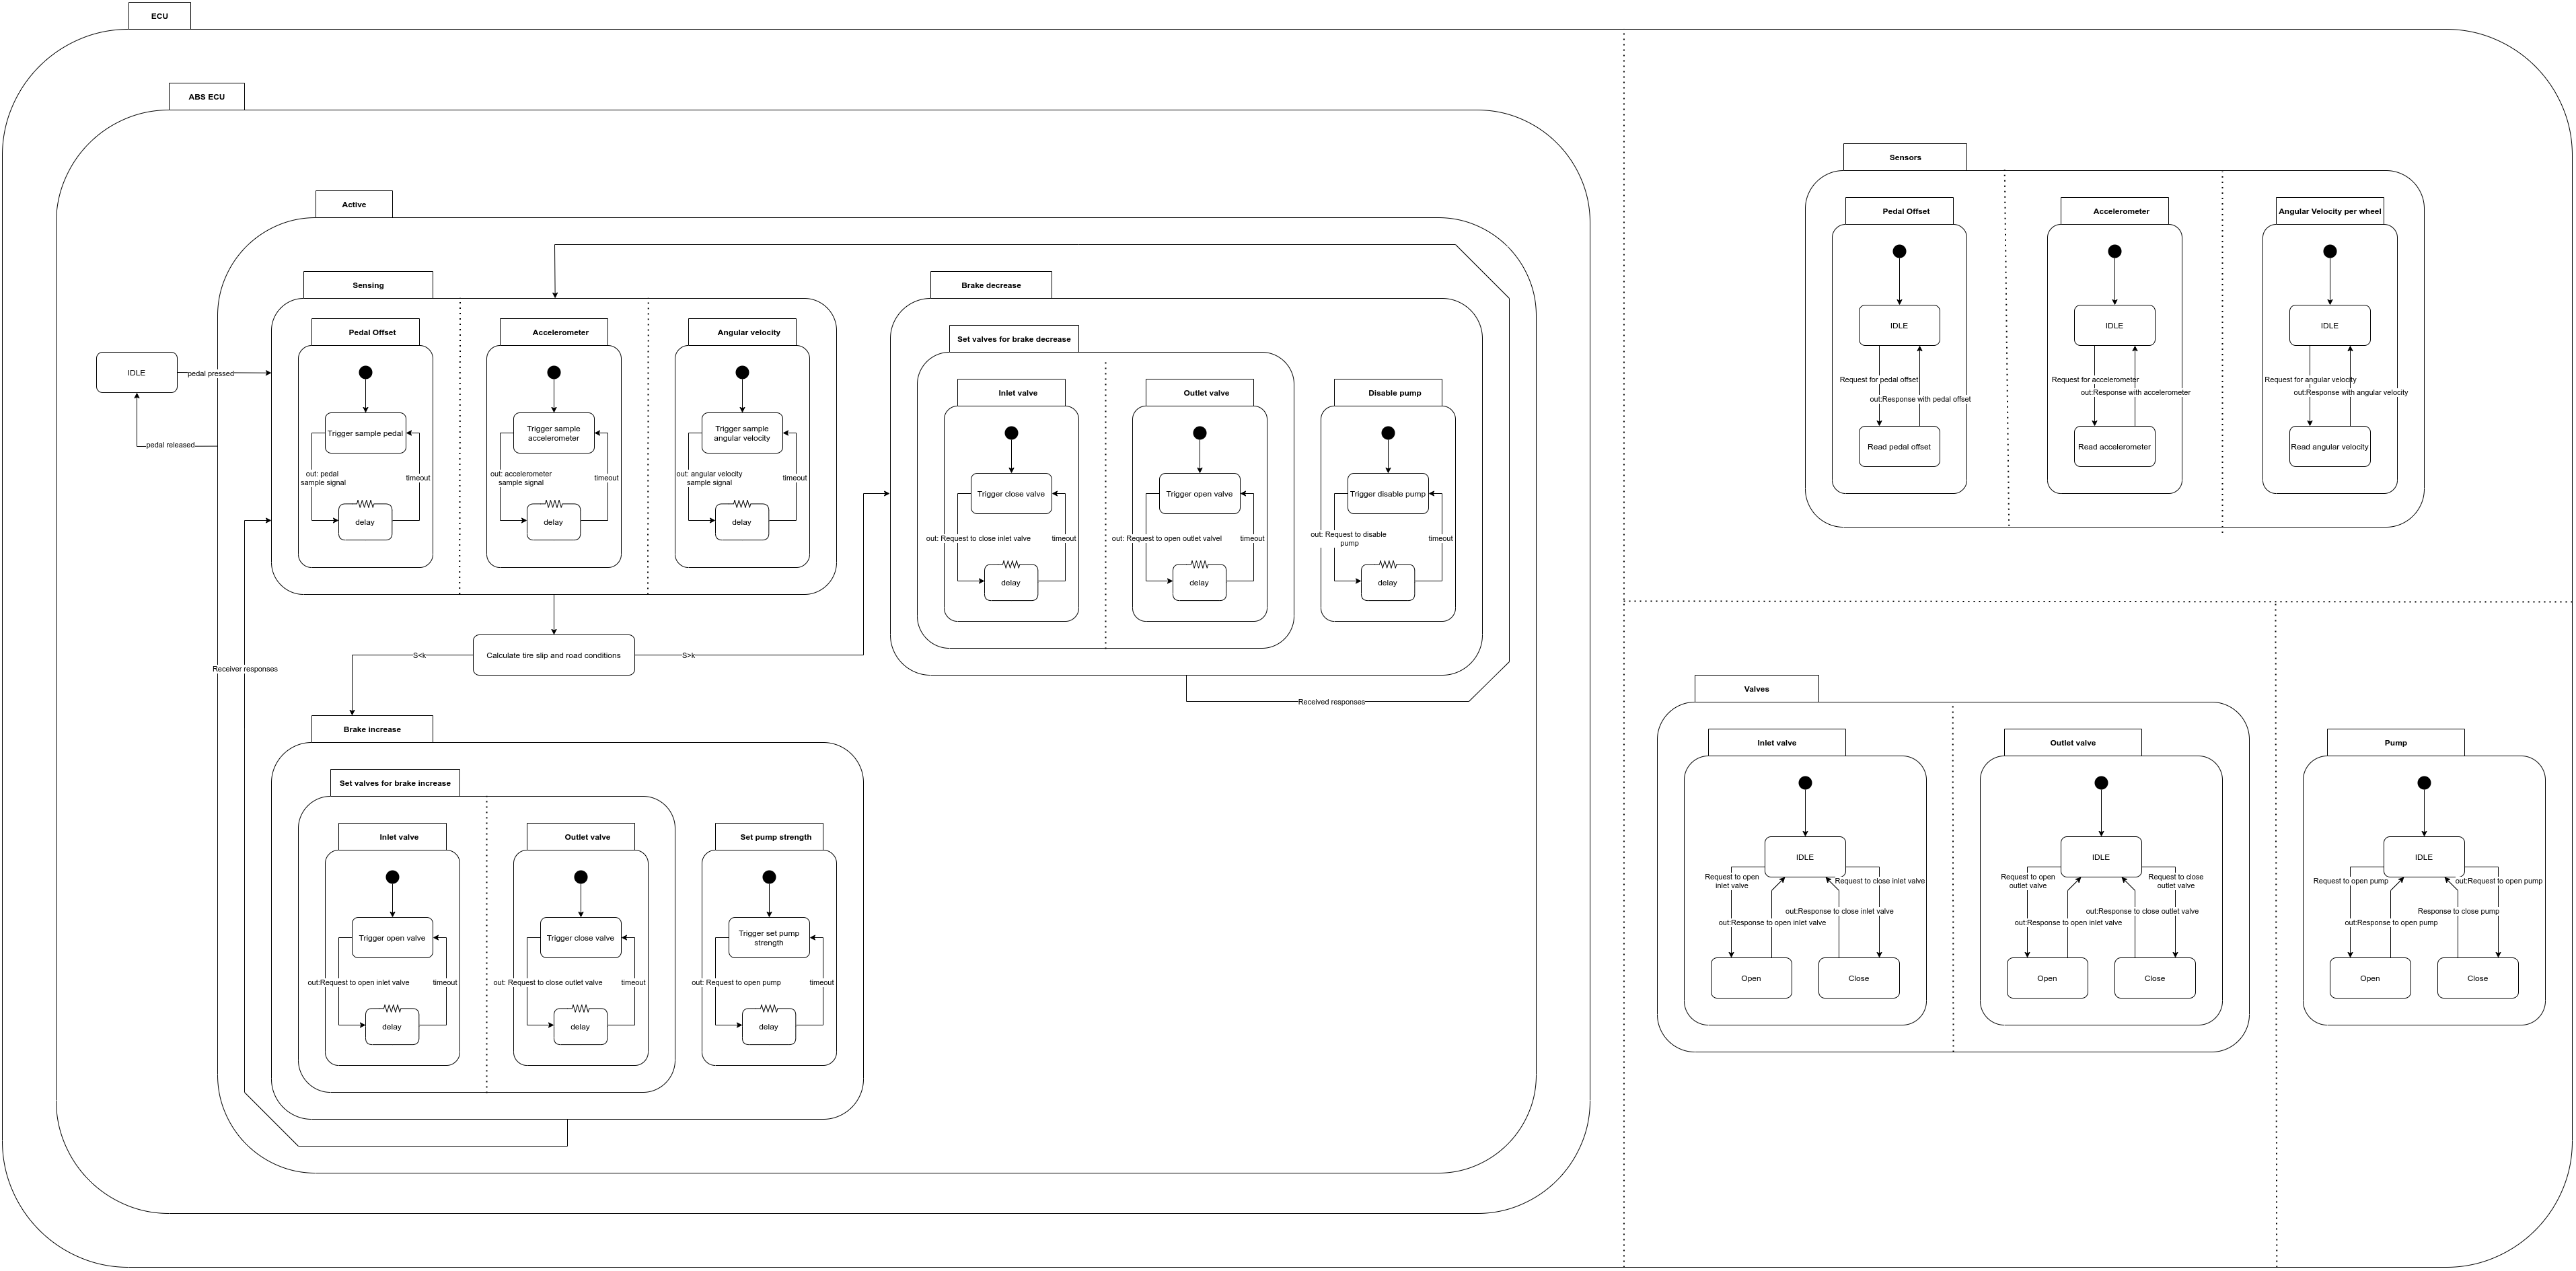
\includegraphics[angle=90,origin=c,scale=0.14]{images/system-architecture-detailed.png}}
    \caption{Λεπτομερής αρχιτεκτονική του συστήματος με StateChart.}
    \label{fig:system-architecture-detailed}
\end{figure}

\subsection{Αρχιτεκτονική λογισμικού}
Σχετικά με το λογισμικό είναι σχετικά περιορισμένη η ύπαρξη του στα περισσότερα υποσυστήματα. Αυτά που είναι υπεύθυνα για τις εισόδους αναλαμβάνουν να διαβάζουν τις τιμές των αισθητήρων και να τις μεταφέρουν στην ECU και αυτά των εξόδων κάνουν την αντίστροφη διαδικασία. Είναι αρκετά απλές διεργασίες. Ο περισσότερος όγκος λογισμικού βρίσκεται στην διαδικασία επικοινωνίας της ECU με τα άλλα υποσυστήματα και στον αλγόριθμο λήψης των αποφάσεων από την ECU. Αρκετά αφαιρετικά η λειτουργία της φαίνεται στο Σχήμα \ref{fig:system-sequence-diagram}. Σχετικά με τον αλγόριθμο λήψης αποφάσεων από την ECU, δεν γνωρίζουμε κάποια υλοποίηση του στη βιβλιογραφία σε υλικό μέχρι στιγμής, για αυτό επιλέγουμε να τον υλοποιήσουμε σε λογισμικό. Σχετικά με την επικοινωνία, επειδή έχουμε επιλέξει να έχουμε ένα μεγάλο δίαυλο επικοινωνίας στον οποίο συνδέονται πολλά συστήματα θα χρειαστούμε κάποιο πρωτόκολλο που υλοποιείται σε λογισμικό. Η αρχιτεκτονική λογισμικού βρίσκεται πολύ κοντά στην αρχική της προσέγγιση όπως φαίνεται και στο Σχήμα \ref{fig:software-architecture-detailed}.

\begin{figure}[H]
    \makebox[\textwidth][c]{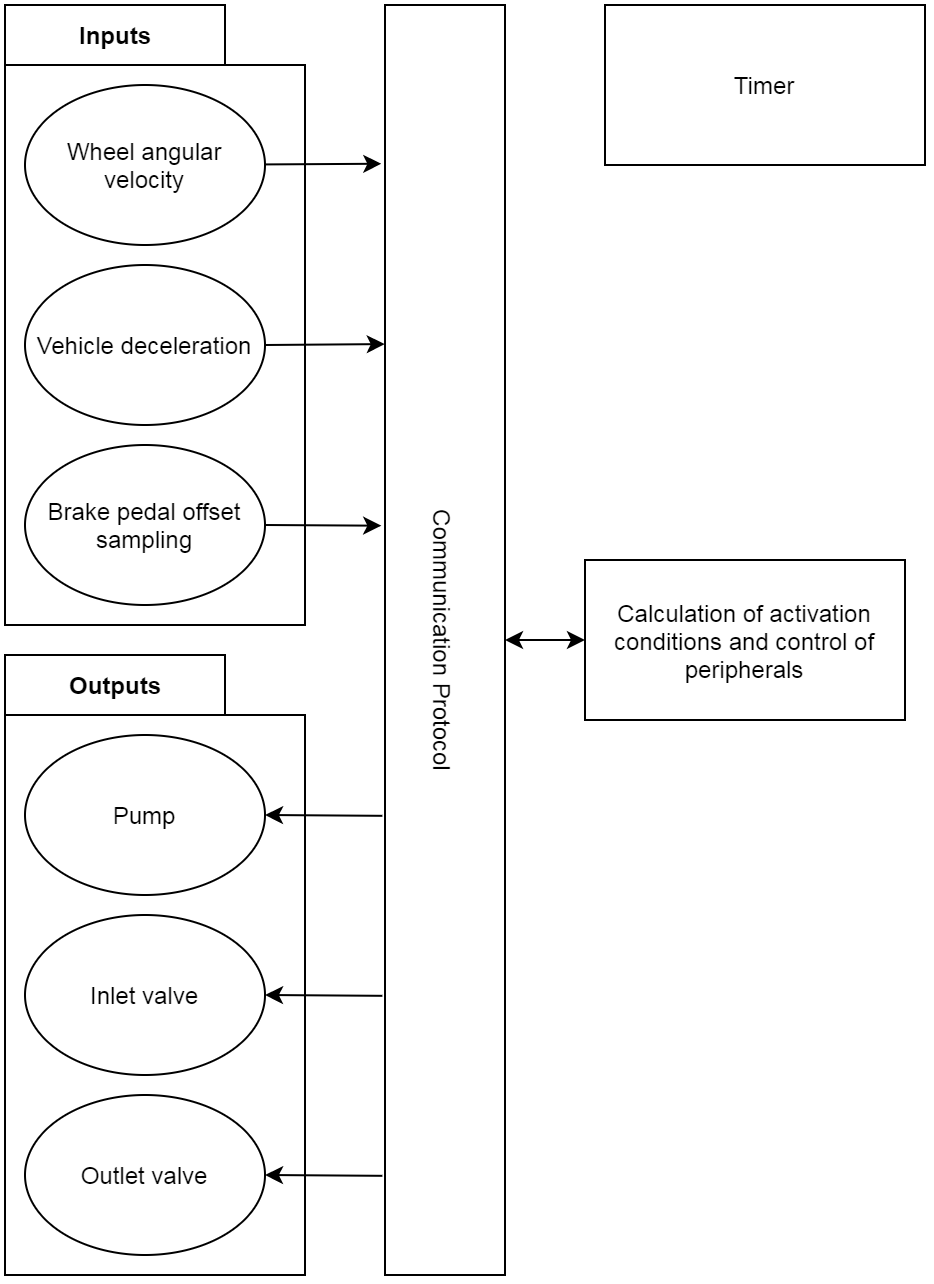
\includegraphics[scale=0.20]{images/software-architecture.png}}
    \caption{Αρχιτεκτονική λογισμικού.}
    \label{fig:software-architecture-detailed}
\end{figure}

\begin{figure}[h]
    \makebox[\textwidth][c]{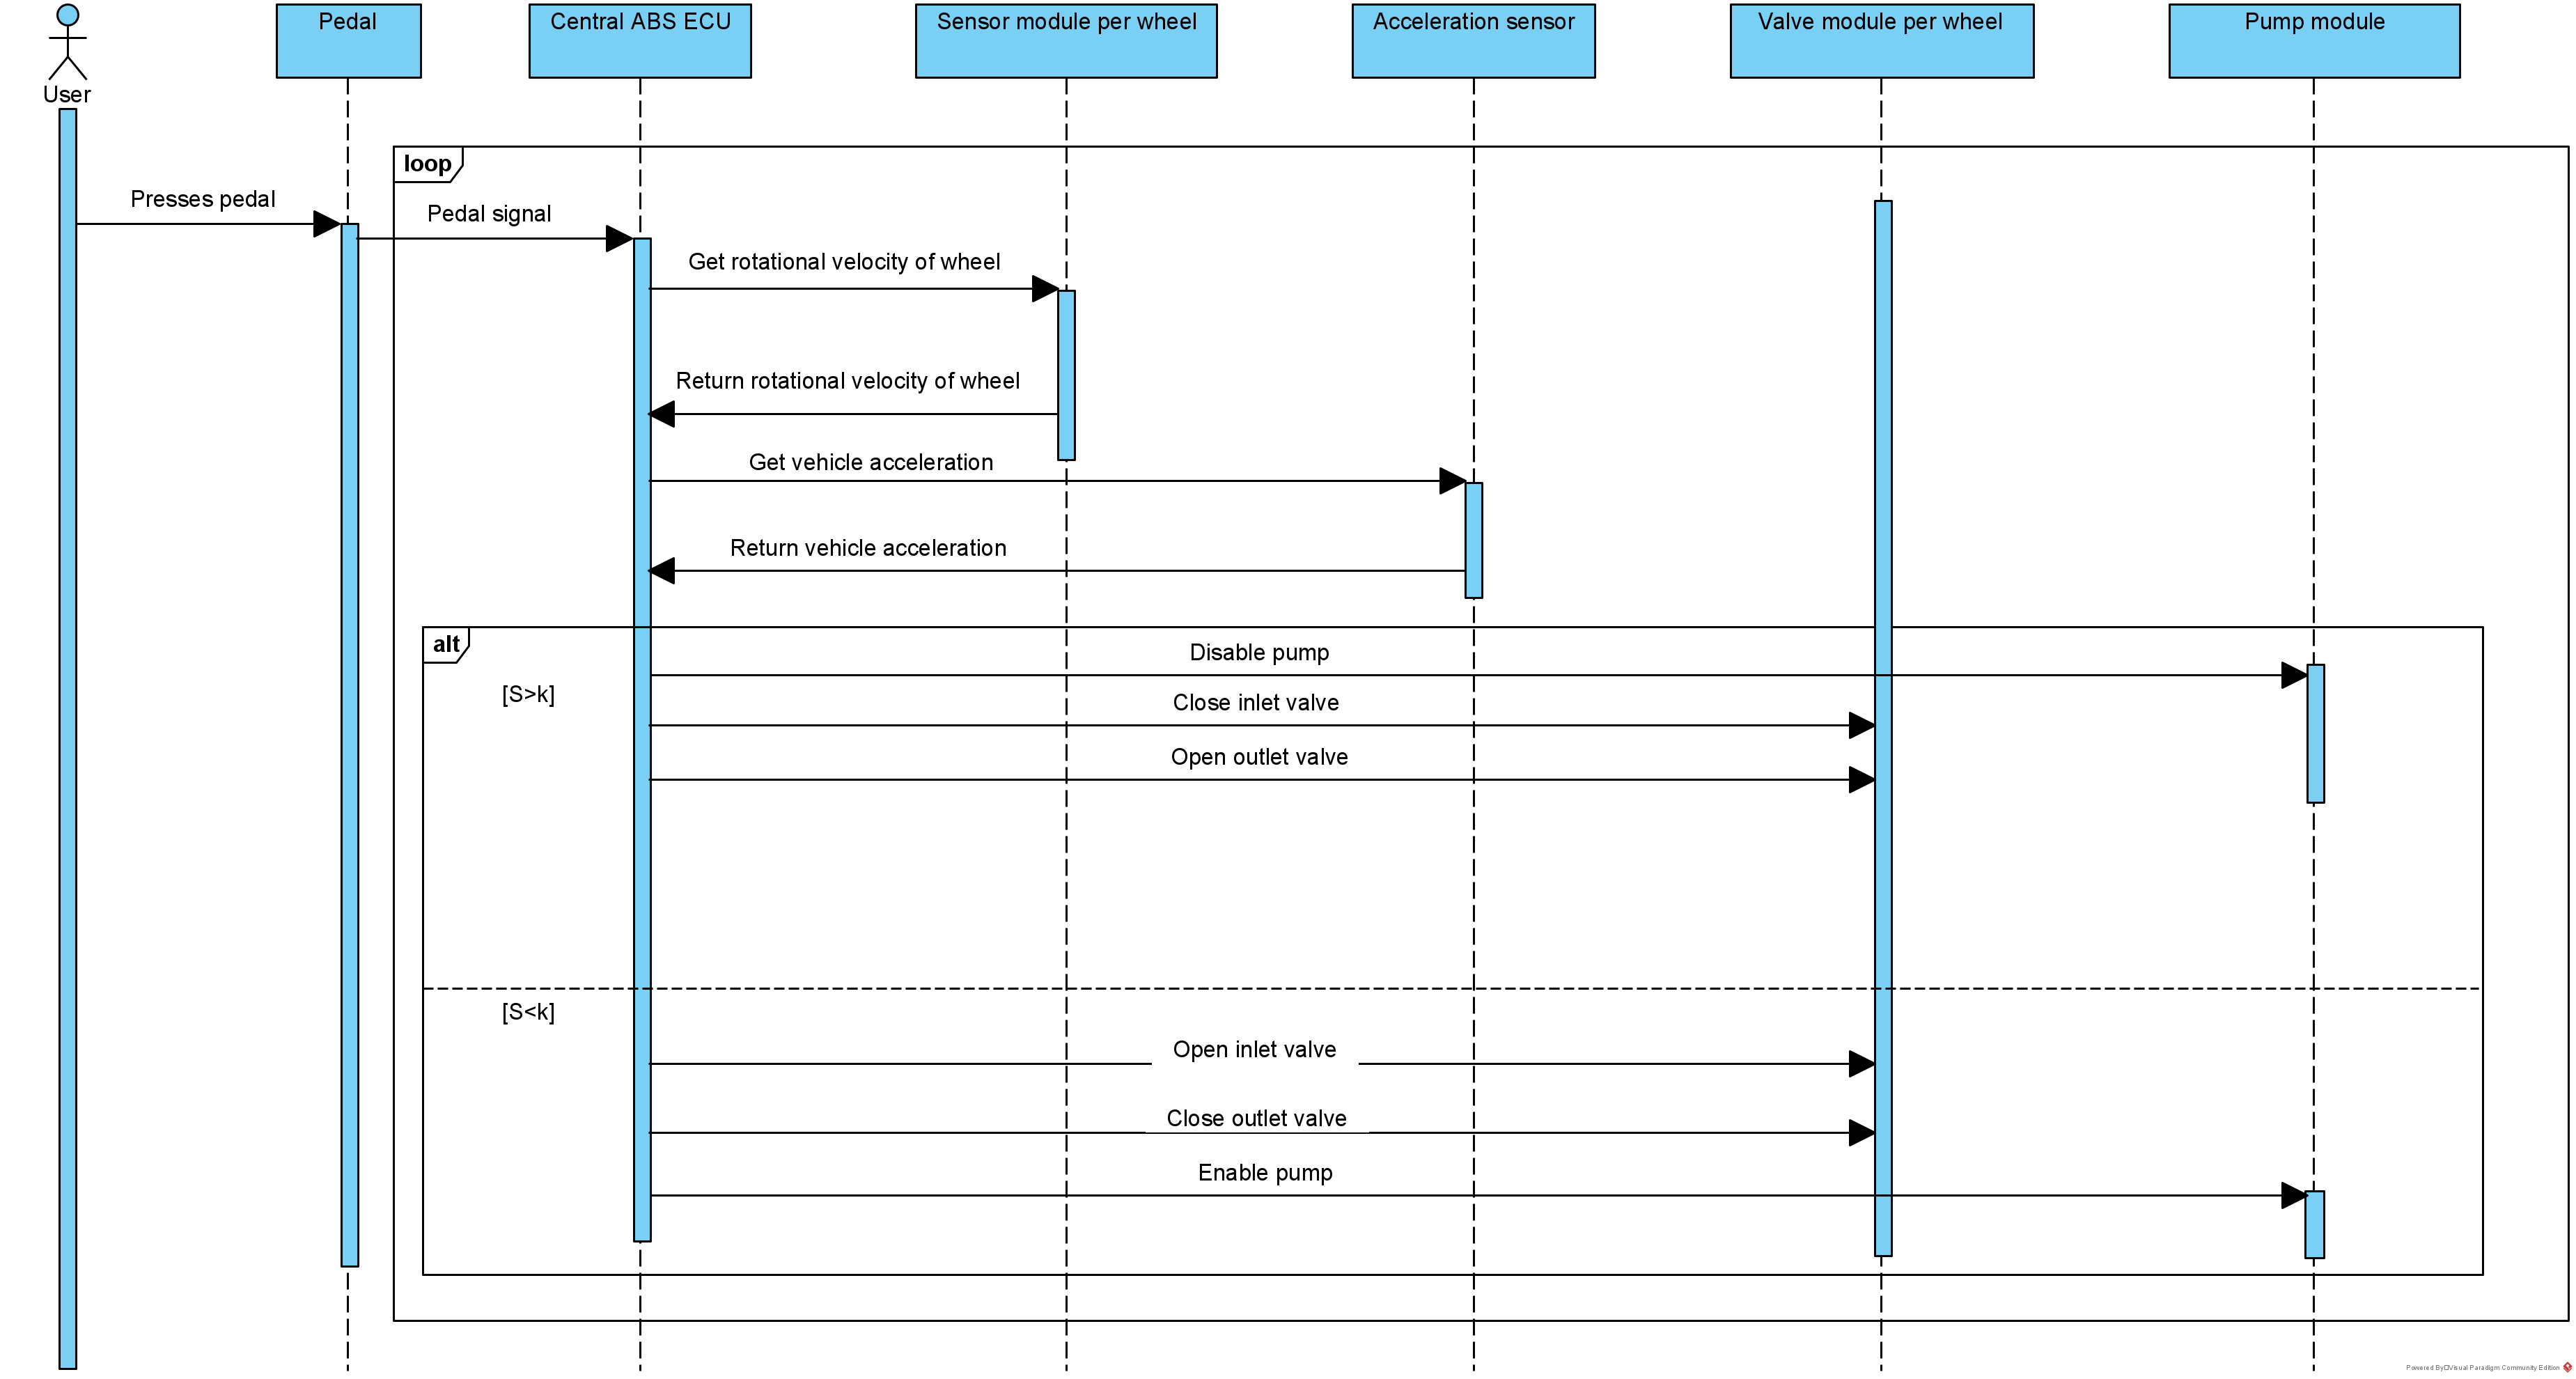
\includegraphics[scale=0.50]{images/system-sequence-diagram.png}}
    \caption{Sequence diagram του συστήματος.}
    \label{fig:system-sequence-diagram}
\end{figure}

\subsection{Αρχιτεκτονική υλικού}
Αρχικά, το σύστημα απαιτεί ένα κεντρικό σημείο συσσώρευσης των εισόδων και υπολογισμού των εξόδων, η φύση του προβλήματος δεν επιτρέπει κάποια κατανεμημένη αρχιτεκτονική, γι' αυτό έχουμε ένα κεντρικό κόμβο, την ECU. Ιδανικά θα θέλαμε κάθε κόμβος να έχει το δικό του κανάλι επικοινωνίας με την ECU ώστε να μπορεί να επικοινωνεί άμεσα με αυτή. Αυτό θα μπορούσε να συμβεί αν υιοθετούσαμε κάποιο ασύρματο τρόπο επικοινωνίας, ωστόσο αποτελεί μια αναξιόπιστη λύση. Μια άλλη λύση, θα ήταν οι αισθητήρες (είσοδοι) να συνδέονταν από κοινού σε έναν δίαυλο επικοινωνίας και οι actuators σε έναν ξεχωριστό. Αυτή η σχεδιαστική επιλογή έχει επιλεγεί από διάφορους κατασκευαστές ABS στο παρελθόν, ωστόσο στη περίπτωση μας δεν μας προσφέρει κάποιο κέρδος καθώς έχουμε έναν σύγχρονο αλγόριθμο στον οποίο η είσοδος και η έξοδος δεν μπορούν να λειτουργήσουν ταυτόχρονα. Έτσι, επιλέξαμε όλα τα συστήματα να επικοινωνούν από κοινού με ένα δίαυλο, για αυτό και κάθε υποσύστημα διαθέτει έναν ελεγκτή διαύλου. Λαμβάνοντας υπόψιν την απλούστευση ότι θα χρειαστούμε έναν αισθητήρα σε κάθε τροχό, η αρχιτεκτονική του αμαξιού μας επιβάλει να χρησιμοποιήσουμε 4 υποσυστήματα αισθητήρων. Σχετικά με το υποσύστημα των βαλβίδων, η επιλογή αυτής της αρχιτεκτονικής έχει να κάνει περισσότερο με τα υδραυλικά και ηλεκτρικά μέρη του συστήματος, των οποίων η ανάλυση είναι εκτός των σκοπών αυτής της εργασίας. Αρκούμαστε, στο ότι στα περισσότερα αυτοκίνητα όλες οι βαλβίδες είναι συγκεντρωμένες σε ένα σημείο. Τέλος σχετικά με το πεντάλ και την αντλία έχουν επιλεχθεί οι πιο απλές αρχιτεκτονικές λαμβάνοντας υπόψιν το τι επιλέξαμε για τα υπόλοιπα συστήματα. 

\begin{figure}[h]
    \begin{center}
    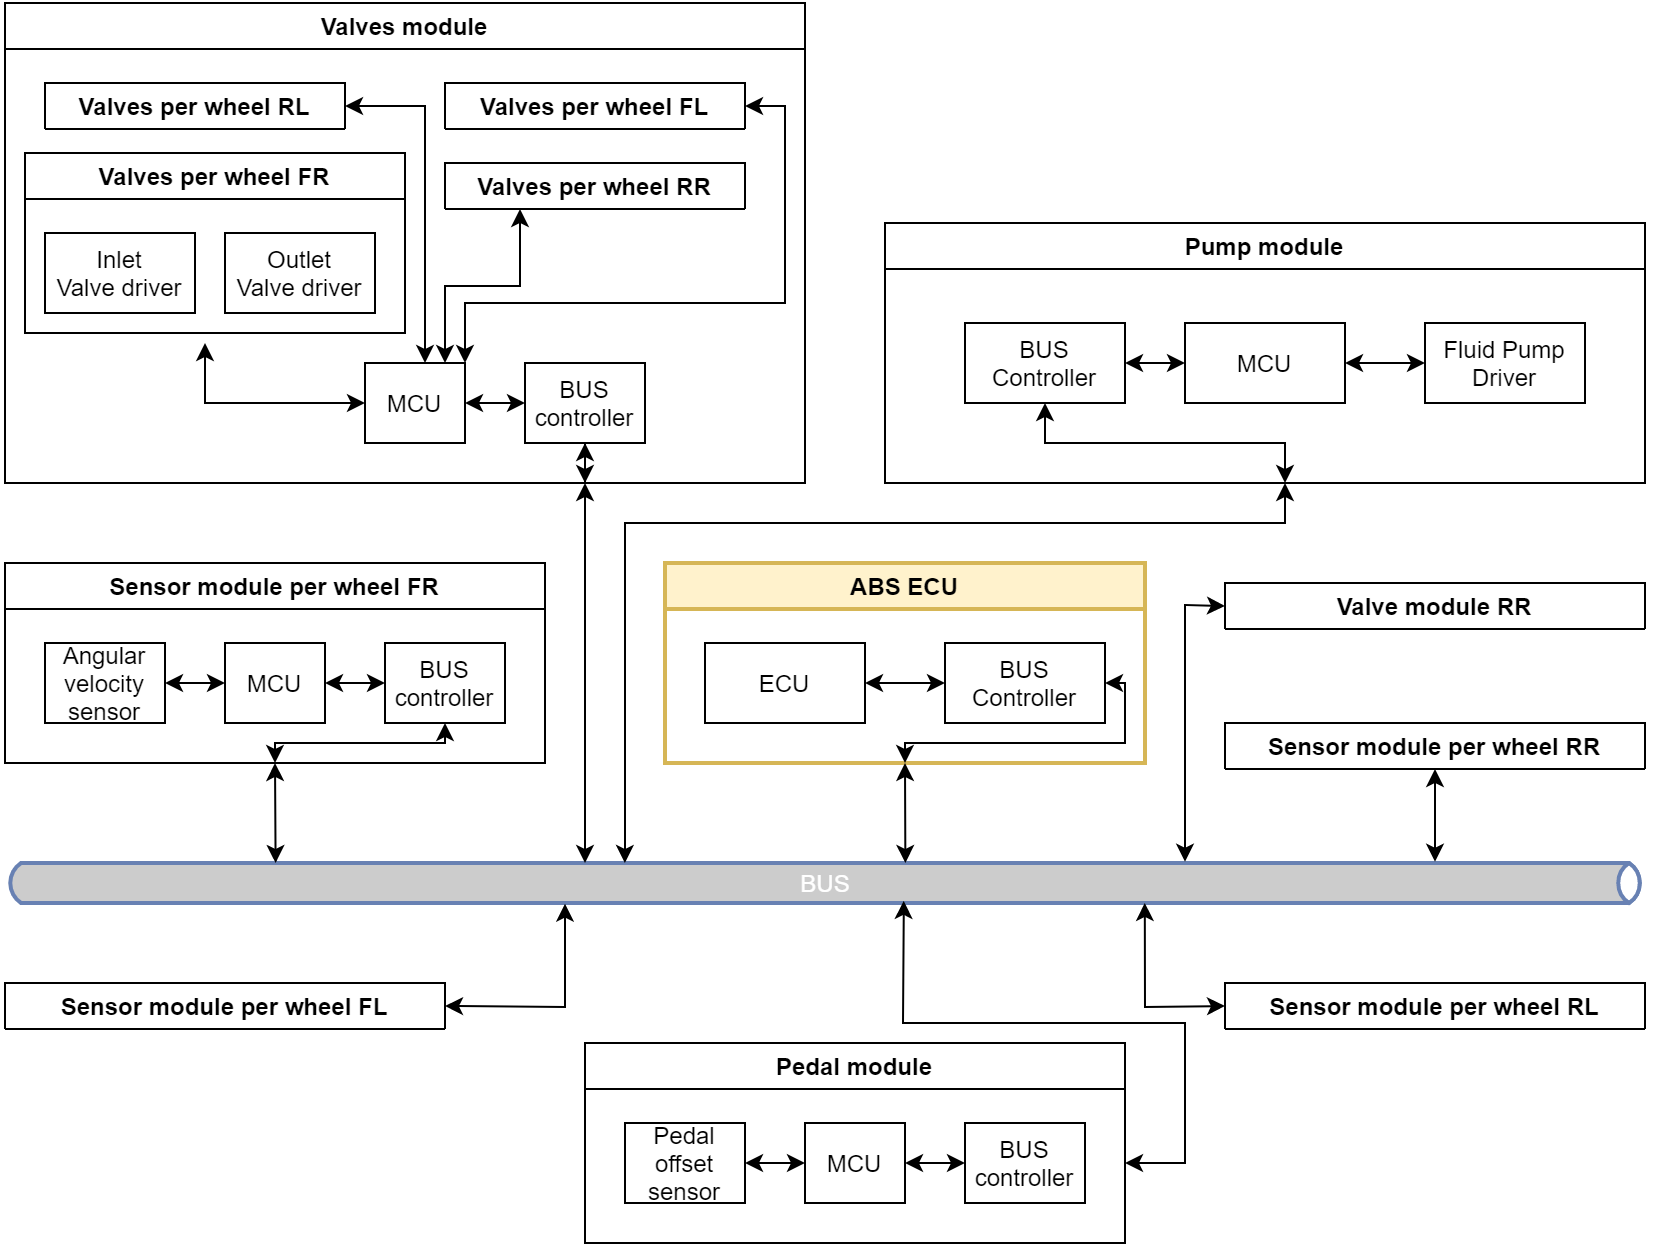
\includegraphics[scale=0.2]{images/hardware-architecture.png}
    \end{center}
    \caption{Αρχιτεκτονική υλικού του συστήματος.}
    \label{fig:hardware-architecture}
\end{figure}

\section{Σχεδιασμός υποσυστημάτων}

\subsection{Υποσύστημα δίαυλου επικοινωνίας}
Επιλέχθηκε ο δίαυλος Controller Area Network (CAN) \cite{can20} για την επικοινωνία των μερών του συστήματος μας, γιατί ανταπεξέρχεται στις προδιαγραφές που έχουμε θέσει. Πρόκειται για ένα δίαυλο που υπάρχει στα περισσότερα αυτοκίνητα σήμερα και προτιμάται από πολλούς κατασκευαστές για τον συγχρονισμό και έλεγχο των μηχανικών μερών και άρα το σύστημα μας μπορεί να τοποθετηθεί σχετικά εύκολα σαν επέκταση της παρούσας υποδομής. Υλοποιείται σε 2 επίπεδα, στο φυσικό επίπεδο που ορίζει τα χαρακτηριστικά και την αρχιτεκτονική του διαύλου και στο επιπέδου μετάδοσης δεδομένων, που ορίζει το πρωτόκολλο. Χαρακτηριστικά είναι ανεκτικός στο θόρυβο μιας και χρησιμοποιεί διαφορική μετάδοση δεδομένων στο φυσικό επίπεδο και για αυτό τον προτιμούμε έναντι άλλων διαύλων π.χ. I\textsuperscript{2}C. Επίσης, μπορεί να υποστηρίξει bitrate εώς και 1Mbps ωστόσο αυτή είναι μια μέτρηση σε ένα δίαυλο 30 μέτρων υπό ιδανικές συνθήκες \cite{canreq:20}. Στη πραγματικότητα το bitrate εξαρτάται εξαρτάται από παράγοντες όπως το μήκος του δίαυλου, τον συνολικό αριθμό των κόμβων που επικοινωνούν μέσω αυτού, τον τύπο τον πομποδεκτών κτλ. Μιας τέτοιας τάξης ρυθμός ικανοποιεί της απαιτήσεις της εφαρμογής μας χωρίς να του προκαλεί κορεσμό όπως θα αναλύσουμε παρακάτω. Δεν απαιτεί κεντρικό συντονισμό που απαιτούν δίαυλοι με αρχιτεκτονική master-slave όπως ο LIN και ο Flexray. Χρησιμοποιεί CSMA/CA αποφεύγοντας τις συγκρούσεις με τη χρήση προτεραιοτήτων το οποίο αποτελεί βασική απαίτηση ενός hard real-time συστήματος όπως το ABS. Στο Σχήμα \ref{fig:vehicle-buses-overview} υπάρχει μια σύγκριση μεταξύ αυτών των διαύλων. Τέλος, μια ακόμα ενδιαφέρουσα επιλογή αν είχαμε επιλέξει αρχιτεκτονική με ξεχωριστό δίαυλο για τους αισθητήρες και ξεχωριστό για τους actuators θα ήταν ο δίαυλος Peripheral Sensor Interface 5 (PSI5) για τους αισθητήρες, για τους actuators θα μπορούσαμε να χρησιμοποιήσουμε κάποιον προϋπάρχον. Τέτοιες επιλογές ανεβάζουν το κόστος αλλά μπορεί να βοηθήσουν στη ελάφρυνση κάποιου υπερφορτωμένου διαύλου.
\par
Ιδανικά θα επιθυμούσαμε το κάθε συστατικό αισθητήρα ή actuator να επικοινωνεί απευθείας με την ECU μέσω του διαύλου. Ωστόσο αυτό δεν είναι εφικτό λόγω της φύσης του CAN και για αυτό σε κάθε αισθητήρα ή actuator προσθέτουμε έναν ελεγκτή διαύλου και έναν μικροελεγκτή. Κάθε υποσύστημα μας διαθέτει αυτά τα δύο συστατικά. Προς το παρόν, θα τα θεωρούμε ίδια για κάθε υποσύστημα με εξαίρεση αυτό της ECU και θα τα αναλύσουμε εδώ αντί να τα αναλύουμε επιμέρους σε κάθε υποσύστημα. O μικροελεγκτής έχει την δυνατότητα να επικοινωνεί μέσω του κεντρικού δίαυλου του συστήματος με την ECU. Για την επικοινωνία με τον ελεγκτή διαύλου CAN, επειδή θα βρίσκονται αρκετά κοντά θα μπορούσαμε να χρησιμοποιήσουμε κάποιο από τα συνήθη πρωτόκολλα και τους αντίστοιχους διαύλους, πιθανότατα SPI ή I\textsuperscript{2}C. Αυτό εισάγει δύο παραπάνω συστατικά στο σύστημα, ωστόσο και αυτά συνηθίζεται να ενσωματώνονται πλέον στους περισσότερους μικροελεγκτές. Σχετικά με τον ελεγκτή διαύλου CAN αυτός αποτελείται από δύο συστατικά, λόγω των 2 επιπέδων στα οποία υλοποιείται το CAN. Πιο συγκεκριμένα τον ελεγκτή που είναι υπεύθυνος για το πρωτόκολλο και τον πομποδέκτη (transceiver) που είναι υπεύθυνος για το φυσικό επίπεδο.

\begin{figure}[H]
    \begin{center}
    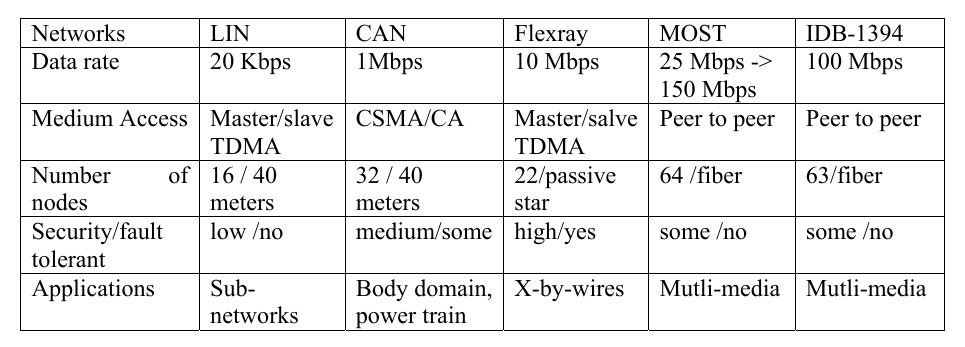
\includegraphics[scale=0.44]{images/vehicle-buses-overview.png}
    \end{center}
    \caption{Σύγκριση διαδεδομένων διαύλων επικοινωνίας που χρησιμοποιούνται στα αυτοκίνητα \cite{Nouvel2009AutomotiveNA}.}
    \label{fig:vehicle-buses-overview}
\end{figure}

\subsubsection{Μέγιστοι ρυθμοί μετάδοσης}
Παρακάτω θα προσπαθήσουμε να κάνουμε μια θεωρητική εκτίμηση της χρήσης του διαύλου CAN από το σύστημα μας θεωρώντας στο μοντέλο μας πως η ταχύτητα του εξαρτάται μόνο από το μήκος του διαύλου, όπως στο Σχήμα \ref{fig:can-latencies}. Η συχνότητα λειτουργίας του συστήματος μας όπως έχουμε αναφέρει στις προδιαγραφές είναι 10 φορές το δευτερόλεπτο, δηλαδή για ένα τροχό, μέσα σε ένα δευτερόλεπτο το ABS μπορεί να πραγματοποιήσει 10 διορθωτικές κινήσεις που κάθε μια από αυτές μπορεί είτε να αυξάνει την πίεση (στα τακάκια) είτε να την μειώνει, αυξάνοντας ή μειώνοντας το ποσοστό ολίσθησης αντίστοιχα. Για να πραγματοποιήσουμε τις διορθωτικές κινήσεις στους τροχούς, χρειάζεται να γίνουν υπολογισμοί και να επικοινωνήσουν τα υποσυστήματα με την ABS ECU. Στη συνέχεια θα περιγράψουμε ένα μοντέλο αξιολόγησής του διαύλου κάνοντας απλουστεύσεις και λαμβάνοντας υπόψιν τη χείριστη περίπτωση. Δεν λαμβάνουμε υπόψιν ότι μπορεί να υπάρχουν και άλλα υποσυστήματα εκτός του κυκλώματος μας που να εκπέμπουν στο δίαυλο γιατί θεωρούμε πως η επικοινωνία του υποσυστήματος μας έχει ύψιστη προτεραιότητα.
\par
Οι υπολογισμοί απαιτούν ως είσοδο δεδομένα από τον αισθητήρα στο πεντάλ του φρένου που μετράει την μετατόπιση και έχει μέγεθος 4 bytes, από τον αισθητήρα επιτάχυνσης (επιταχυνσιόμετρο) που θεωρούμε πως έχουν μήκος 4 bytes και από τους αισθητήρες γωνιακής ταχύτητας που θεωρούμε πως έχουν μήκος (4 bytes) * 4 (για όλους τους τροχούς). Αφού πραγματοποιηθεί ο υπολογισμός, η ABS ECU θα στείλει μηνύματα με προορισμούς τις βαλβίδες και την αντλία. Για να ελέγξουμε τις βαλβίδες απαιτείται 1 byte (τα πρώτα 4 bit είναι σημαίες για τις βαλβίδες εισόδου και τα επόμενα για τις βαλβίδες εξόδου) και για την αντλία 4 bytes. Όπως φαίνεται και στο σχήμα \ref{fig:inner-communications}.

\begin{figure}[H]
\makebox[\textwidth][c]{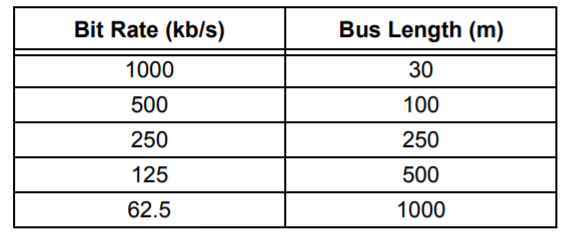
\includegraphics[scale=0.3]{images/can-bus-latencies.png}}
\caption{Μέγιστo bitrate ανά μήκος διαύλου, στον δίαυλο CAN \cite{canreq:20}}
\label{fig:can-latencies}
\end{figure}

\begin{figure}[H]
\makebox[\textwidth][c]{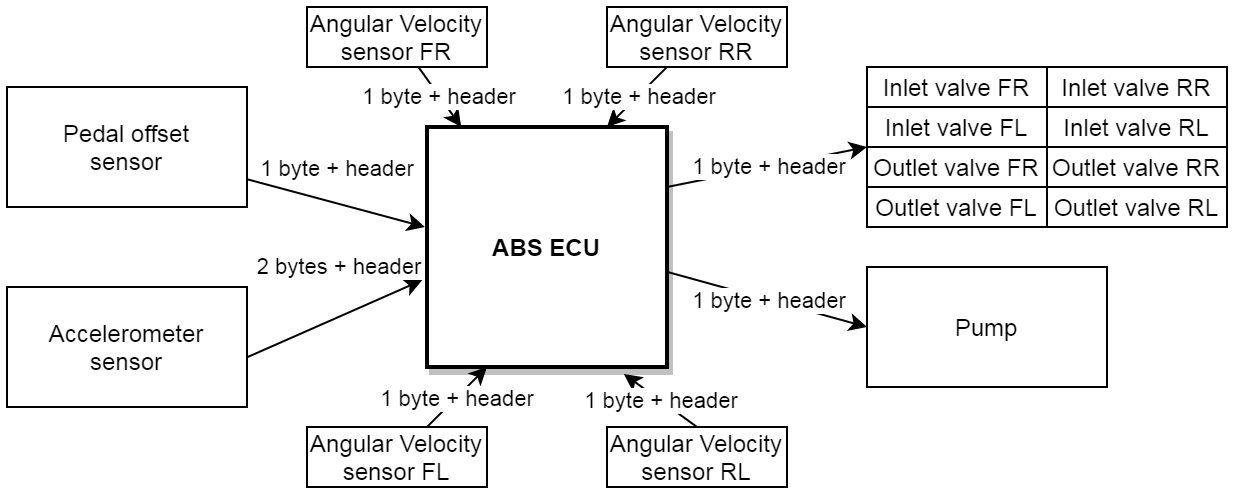
\includegraphics[scale=0.3]{images/inner-communications-v2.png}}
\caption{Επικοινωνία στον δίαυλο CAN}
\label{fig:inner-communications}
\end{figure}

Αξίζει να παρατηρήσουμε πως οι αισθητήρες γωνιακής ταχύτητας \ref{angular-sensors-module} δεν μπορούν να ομαδοποιήσουν κάπως την πληροφορία που θέλουν να στείλουν, όπως γίνεται για τις οκτώ βαλβίδες, επειδή βρίσκονται σε απόσταση (σε αντίθεση με τις βαλβίδες που βρίσκονται κοντά και μπορεί να χρησιμοποιηθεί κάποιος ενιαίος CAN controller \ref{valves-module}).
\par
Από το σχήμα \ref{fig:inner-communications} προκύπτει πως το συνολικό μέγεθος των δεδομένων που θα μεταφερθούν μέσω CAN BUS θα ισούται με:  
\begin{multline*}Data(\text{Length}) = 1 \text{ byte} + header + 1 \text{ byte} + header + 1 \text{ byte} + \text{ header} + 1 \text{ byte} +\\
header + 1 \text{ byte} + header + 1 \text{ byte} + header + 1 \text{ byte} + header + 2 \text{ bytes} + header\end{multline*}
Στον δίαυλο CAN θεωρούμε \(header=44 \text{ bits}\), οπότε θα έχουμε $Data(\text{Length}) = 53 \text{ bytes}$.
Έχουμε όμως υπολογίσει την φόρτωση του δίαυλου σε ένα κύκλο της λειτουργίας του συστήματος μας.
Οπότε σε 1 δευτερόλεπτο ο συνολικός όγκος δεδομένων που εναλλάσσεστε στον δίαυλο θα είναι:
%\[Data(Length) = 73*10 \frac{bytes}{sec}\]
%\centerline{Ισοδύναμα θα έχουμε:}
\[Data(\text{Length}) = 530 \text{ bytes/sec}\]
\par
Επίσης αφήνουμε αρκετό χώρο στον δίαυλο και για άλλα συστήματα να επικοινωνήσουν με αυτον. Η CAN μπορεί να φτάσει data rates από 200Kbps έως και 1Mbps όπως φαίνεται και στο Σχήμα \ref{fig:vehicle-buses-overview} ωστόσο αυτό εξαρτάται από πολλούς παράγοντες όπως προαναφέραμε. Στέλνουμε 4240 bits το δευτερόλεπτο οπότε χρησιμοποιούμε το δίαυλο στο 2.12\% στα 200kbps και 0.4\% στο 1Mpbs. Άρα η χρήση του Controller Area Network (CAN) είναι κατάλληλη για το σύστημά μας.

\subsection{Υποσύστημα αισθητήρα τροχού}\label{angular-sensors-module}
Ο σκοπός του υποσυστήματος μας είναι να μπορεί ενημερώνεται κεντρική ECU με τις γωνιακές ταχύτητες όλων των τροχών πριν κρίνει ποιος τροχός πρέπει να ολισθήσει περισσότερο ή λιγότερο. Το υποσύστημα αισθητήρα τροχού υπάρχει ξεχωριστό για κάθε τροχό. Θα το αναλύσουμε για έναν τροχό. Αποτελείται από έναν αισθητήρα, έναν μικροελεγκτή και ένα ελεγκτή διαύλου. Ο αισθητήρας μπορεί να μετράει την γωνιακή ταχύτητα στους τροχούς και έχει σήμα εξόδου για αποστολή δεδομένων και σήμα εισόδου για έλεγχο του. Ο μικροελεγκτής μπορεί (με την βοήθεια του μικροελεγκτή διαύλου) να επικοινωνεί με την ECU του συστήματος, να δειγματοληπτεί τον αισθητήρα ανάλογα με το πως αποφασίζει αυτή σύμφωνα με την αρχιτεκτονική λογισμικού, καθώς και πιθανόν να τον ρυθμίζει. Ανάλογα με τη φύση του αισθητήρα, ίσως χρειαστούμε και ένα συστατικό που να μετατρέπει το σήμα του. Πολλές φορές αυτοί οι μηχανισμοί είναι ενσωματωμένοι στον μικροελεγκτή. Ο μικροελεγκτής διαύλου γεφυρώνει τον κεντρικό δίαυλο με τον μικροελεγκτή του υποσυστήματος μας και αναλύθηκε παραπάνω.

\begin{figure}[H]
\makebox[\textwidth][c]{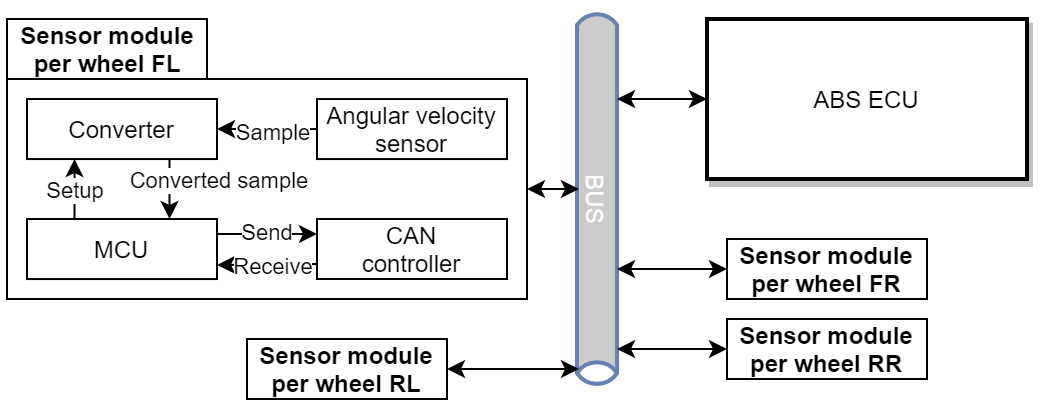
\includegraphics[scale=0.30]{images/angular-velocity-module-design.png}}
\caption{Σχηματική αναπαράσταση υποσυστήματος αισθητήρων γωνιακής ταχύτητας}
\label{fig:sensors-module}
\end{figure}

\subsection{Υποσύστημα πεντάλ φρένου}
Το πεντάλ φρένου δεν διαφέρει ιδιαίτερα από τον αισθητήρα γωνιακής ταχύτητας τροχού πέρα από τη φύση του αισθητήρα και γι' αυτό δεν θα το αναλύσουμε.

\subsection{Υποσύστημα βαλβίδων}\label{valves-module}
Ο σκοπός του υποσυστήματος μας είναι η κεντρική ECU να μπορεί να ελέγχει μέσω επικοινωνίας με τον δίαυλο όλες τις βαλβίδες. Το υποσύστημα αισθητήρα βαλβίδων περιέχει συνολικά τέσσερις βαλβίδες εισόδου και τέσσερις βαλβίδες εξόδου, έναν μικροελεγκτή και ένα ελεγκτή διαύλου. Οι βαλβίδες αποτελούν μέρη του συστήματος τα οποία δεν θα αναλύσουμε. Ο μικροελεγκτής μπορεί να ελέγχει όλες τις βαλβίδες και με την βοήθεια του μικροελεγκτή διαύλου να επικοινωνεί με την κεντρική δίαυλο του συστήματος λαμβάνοντας οδηγίες από την κεντρική ECU. Για τον χειρισμό των βαλβίδων από τον μικροελεγκτή πιθανότατα να χρειαστεί η επικοινωνία με κάποιο συστατικό ελέγχου τους και άρα και κάποιο πρωτόκολλο επικοινωνίας τους.

\subsection{Υποσύστημα αντλίας}
Ο σκοπός του υποσυστήματος μας είναι ρύθμιση της αντλίας από την ECU. Η αρχική σχεδίαση είναι πως το υποσύστημα αντλίας αποτελείται από έναν μικροελεγκτή και μια αντλία και έναν ελεγκτή διαύλου ο οποίος αναλύθηκε παραπάνω. Μετά από λεπτομερέστερη εξέταση προκύπτουν και άλλα συστατικά που θα χρειαστούν. Ξεκινώντας από την αντλία, η ανάλυση των υδραυλικών και μηχανικών μερών της δεν μας αφορά. Μπορούμε να την θεωρήσουμε σαν ένα μοτέρ. Σίγουρα θα χρειαστεί κάποιος οδηγός της αντλίας και στη πλευρά του μικροελεγκτή που οδηγεί την αντλία κάποιο συστατικό το οποίο να επικοινωνεί με αυτόν. Μια συνήθης μέθοδος ελέγχου που χρησιμοποιείται για αυτούς τους σκοπούς είναι το Pulse Width Modulation (PWM), η οποία μας επιτρέπει να ρυθμίσουμε και το πόσο δυνατά θα δουλεύει η αντλία. Κυκλώματα που να υλοποιούν αυτή τη μέθοδο συνήθως είναι ενσωματωμένα και στους πιο φθηνούς μικροελεγκτές.

% \begin{figure}[H]
% \makebox[\textwidth][c]{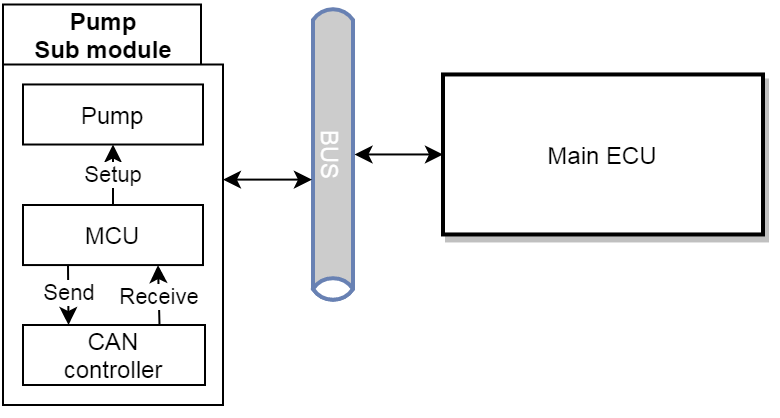
\includegraphics[scale=0.35]{hardware-architecture-preview-Pump-submodule.png}}
% \caption{Εικονική αναπαράσταση υποσυστήματος αντλίας}
% \label{fig:innerCommunications}
% \end{figure}

\subsection{Υποσύστημα ABS ECU}
H ECU είναι το πιο κομβικό υποσύστημα του ABS, λαμβάνει δεδομένα από όλες τις εισόδους της, τα επεξεργάζεται για να παράγει πληροφορίες και με βάση αυτές οδηγεί τις εξόδους της.
Κάτι που δεν φαίνεται στην αρχιτεκτονική υλικού του συστήματος είναι πως εντός του υποσυστήματος της ECU βρίσκεται και το επιταχυνσιόμετρο και πιθανών κάποιο συστατικό που μετατρέπει αυτό το σήμα σε ψηφιακό επειδή αυτοί οι αισθητήρες είναι συνήθως αναλογικοί. Επειδή δεν υπάρχουν χωρικοί περιορισμοί ως προς την τοποθέτηση (δηλαδή σε ποιό σημείο θα τοποθετηθεί επειδή το αυτοκίνητο σε κάθε σημείο του θεωρούμε προσεγγιστικά ότι έχει ίδια επιτάχυνση/επιβράδυνση στον άξονα κίνησης του), το τοποθετήσαμε δίπλα από την ECU για να μην φτιάξουμε ξεχωριστό υποσύστημα και αυξήσουμε το κόστος.
\par
Σχεδιαστικά, διακρίνουμε δύο πιθανά σημεία συμφόρησης τα οποία βρίσκονται στον μιρκοελεγκτή της ECU και πρέπει να τα αναλύσουμε. Πιο συγκεκριμένα, στη συγκέντρωση των εισόδων και στην εκτέλεση του αλγορίθμου λήψης απόφασης. Σχετικά με τη συγκέντρωση των εισόδων, το σύστημα μας χρειάζεται να ελέγχει ταυτόχρονα τις εισόδους από 5 διαφορετικά υποσυστήματα, 1 υποσύστημα πεντάλ, 4 υποσυστήματα γωνιακής ταχύτητας καθώς και από το επιταχυνσιόμετρο. Επίσης χρειάζεται να κάνει ταυτόχρονα δειγματοληψία. Αυτό είναι μια πολύ σημαντική ιδιότητα που θέλουμε να έχει το σύστημα μας καθώς αν γινόταν σειριακά μπορεί όταν κάναμε την τελευταία μέτρηση η πρώτη να ήταν ήδη μη έγκυρη. Με βάση αυτή την ανάγκη ταυτοχρονισμού και λαμβάνοντας υπόψιν τη τάξη κόστους του συστήματος, αποφασίσαμε ότι είναι απαραίτητη η χρήση κάποιου λειτουργικού συστήματος πραγματικού χρόνου (RTOS) στον συγκεκριμένο μικροελεγτή. Για αυτό το λόγω και σε επίπεδο προδιαγραφών αυτός ο μικροελεγκτής θα χρειαστεί να είναι ισχυρότερος από τους υπόλοιπους που βρίσκονται στα άλλα υποσυστήματα. Σχετικά με την εκτέλεση του αλγορίθμου, θα χρειαστούμε κάποιον συνεπεξεργαστή μαθηματικών για την επιτάχυνση της εκτέλεσης του αλγορίθμου μιας και αυτός απαιτεί πράξεις κινητής υποδιαστολής (πολλαπλασιασμών και διαιρέσεων που είναι από τις πιο αργές πράξεις) και ας μη ξεχνάμε πως έχουμε να κάνουμε με ένα σύστημα hard real-time σύστημα.

\begin{figure}[H]
\makebox[\textwidth][c]{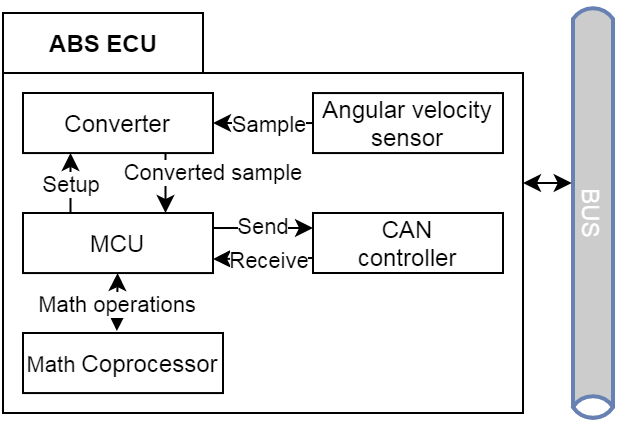
\includegraphics[scale=0.30]{images/central-abs-ecu-module-design.png}}
\caption{Σχηματική αναπαράσταση υποσυστήματος ABS ECU}
\label{fig:sensors-module}
\end{figure}

% \section{Αξιολόγιση σχεδιασμού συστήματος}
% Χρήση Pareto

\section{Σχεδιασμός συστατικών συστήματος/υποσυστημάτων}

\subsection{Συστατικά υποσυστήματος διαύλου επικοινωνίας}
Το υποσύστημα διαύλου επικοινωνίας αποτελείται από τα παρακάτω συστατικά:
\begin{itemize}
    \item Δίαυλος Επικοινωνίας CAN
    \par
    Είναι ο κεντρικός δίαυλος το συστήματος μέσω του οποίου επικοινωνούν όλα τα υποσυστήματα. Εφόσον έχει επιλεγεί το πρότυπο CAN δεν έχουμε σχεδιαστικές επιλογές να κάνουμε αφού είναι standard οι προδιαγραφές του φυσικού επιπέδου σε αυτό. Ο μόνος περιορισμός που έχουμε είναι να έχει όσο είναι εφικτό περισσότερη μόνωση ο δίαυλος γιατί βρίσκεται σε περιβάλλον έντονου ηλεκτρομαγνητικού θορύβου. Το μήκος του διαύλου ποικίλει ανάλογα με τον εφαρμογή ωστόσο θεωρήσουμε ότι είναι στο εύρος των 30-50 μέτρων, δηλαδή μέγεθος που δεν περιορίζει το μέγιστο ρυθμό μετάδοσης σύμφωνα με το Σχήμα \ref{fig:can-latencies}.
    \item Ελεγκτές διαύλου επικοινωνίας
    \par
    Βρίσκονται στο επίπεδο 2 του OSI και υπάρχει ένας σε κάθε υποσύστημα του συστήματος μας και για αυτό το αναλύουμε εδώ διότι δεν έχουμε διαφοροποιήσεις μεταξύ τους. Ιδανικά θα θέλαμε να είναι ενσωματωμένος στον μικροελεγκτή κάθε συστήματος ώστε να μην χρειαστεί να χρησιμοποιήσουμε κάποιο ακόμα πρωτόκολλο (SPI, I\textsuperscript{2}C) για να τον προγραμματίσουμε. Θα θέλαμε επίσης να υποστηρίζει τη μέγιστη ταχύτητα μετάδοσης του 1Mbps λόγω της φύσης του συστήματος. Όπως θα δούμε και στη συνέχεια και τα δυο είναι εφικτά και συνηθίζεται στους περισσότερους σύγχρονους μικροελεγκτές βιομηχανικών σκοπών. Οι ελεγκτές διαύλου θα είναι τα ίδια ολοκληρωμένα για κάθε υποσύστημα.
    \item Πομποδέκτες (transceivers) διαύλου επικοινωνίας
    \par
    Βρίσκονται στο επίπεδο 1 του OSI και υπάρχει ένας σε κάθε υποσύστημα του συστήματος μας και για αυτό το αναλύουμε εδώ διότι δεν έχουμε διαφοροποιήσεις σε αυτό. Επειδή βρίσκεται στο φυσικό επίπεδο σημαίνει πως καθορίζει και αυτός το μέγιστο ρυθμό μετάδοσης. Όπως προαναφέραμε υπάρχει γκάμα επιλογών από 200kbps εώς 1Mbps που υποστηρίζει το πρωτόκολλο. Λόγω της φύσης του συστήματος μας θα επιλέξουμε πομποδέκτη που υποστηρίζει έως και 1Mbps αφού δεν έχει αισθητή διαφορά στο κόστος. Ιδανικά δεν θα θέλαμε το υποσύστημα αυτό να είναι ενσωματωμένο στον μικροελεγτή καθώς εκτός επιτελεί και επιπλέον λειτουργίες προστασίας του συστήματος από επικίνδυνα για το υπόλοιπο κύκλωμα ηλεκτρικά φαινόμενα. Αυτό το καθιστά σχετικά αναλώσιμο και θα θέλαμε να βρίσκεται εκτός του ολοκληρωμένου του μικροελεγκτή ώστε να μπορεί να αλλαχτεί σε περίπτωση βλάβης, ώστε το σύστημα μας να είναι εύκολο στη συντήρηση. Οι πομποδέκτες θα είναι τα ίδια ολοκληρωμένα για κάθε υποσύστημα.
    \item Λογισμικό διαύλου επικοινωνίας
    Σε επίπεδο λογισμικού απαιτούμε μια ελαφριά και κυρίως γρήγορη βιβλιοθήκη η οποία θα τρέχει σε όλους τους μικροελεγκτές ώστε να μπορούν να ελέγχουν ο καθένας τον δικό του Ελεγκτή Διαύλου Επικοινωνίας. 
\end{itemize}

\subsection{Συστατικά υποσυστήματος αισθητήρα τροχού}
Το υποσύστημα αποτελείται από τα παρακάτω συστατικά:
\begin{itemize}
\item Αισθητήρας τροχού
    \par
    Γενικά οι αισθητήρες τροχού παράγουν έναν παλμό που η συχνότητα του αντιστοιχίζεται γραμμικά με την γωνιακή ταχύτητα. Η γωνιακή ταχύτητα αντιστοιχίζεται γραμμικά με την ταχύτητα σε κάποιο σημείο της εφαπτομένης της ρόδας. Οπότε μπορούμε να πούμε ότι η συχνότητα του παλμού του αισθητήρα είναι γραμμικά συνδεδεμένη με την ταχύτητα στην επιφάνεια της ρόδας. Για τους σκοπούς μας, μας αρκεί πληροφορία που αντιστοιχεί σε 1 byte για την γωνιακή ταχύτητα του τροχού (αυτή η πληροφορία θα παραχθεί στον μικροελεγκτή μετά από δειγματοληψία και θα καλύπτει το εύρος των γωνιακών ταχυτήτων που αντιστοιχούν σε γραμμική ταχύτητα από 15 Km/h έως 200 Km/h).
\item Μικροελεγκτής
    \par
    Η μέγιστη ταχύτητα που επιτρέπεται να έχει κάποιο όχημα στην ΕΕ είναι 140 km/h. Για να έχουμε ένα περιθώριο απαιτούμε το υποσύστημα να παράγει χρήσιμες πληροφορίες απο 15 Km/h έως τα 200 Km/h. Επιλέγουμε σαν κατώτατο όριο τα 15 Km/h επειδή η καθυστέρηση μεταξύ δύο διαδοχικών παλμών του παλμού του αισθητήρα ξεπερνάει το χρονικό όριο για το οποίο είναι χρήσιμη η πληροφορία. Θα πρέπει ο μικροελεγκτής να είναι αρκετά γρήγορος για να μπορεί να εντοπίζει τις ακμές του παλμού. Ο αισθητήρας παράγει παλμό της μορφής $\text{α} \cdot \text{(ταχύτητα στην επιφάνεια του τροχού)}$ (όπου το $\text{α}$ εξαρτάται από τη φύση του αισθητήρα). Επίσης είναι αναγκαίο να υποστηρίζει hardware interrupts, για καλύτερη απόδοση. Ακόμα απαιτούμε να έχει υποστήριξη 16-bit hardware timer με δυνατότητα μέτρησης σε μs ώστε να μπορούμε να υπολογίζουμε τη γωνιακή ταχύτητα μέσω των παλμών.
 \item Μετατροπέας ADC σήματος αισθητήρα
    \par
    Θέλουμε ο μετατροπέας ADC να είναι ενσωματωμένος στον μικροελεγκτή για να μην αυξήσουμε επιπλέον την πολυπλοκότητα του υποσυστήματος αλλά και για γρηγορότερη επικοινωνία. Χρειάζεται να είναι γρήγορος για να μπορεί να δειγματοληπτεί έναν αισθητήρα που παράγει πολλούς παλμούς για μια δεδομένη γωνιακή ταχύτητα, αν δεν είναι, πρέπει να επιλέξουμε αισθητήρα που παράγει λιγότερους παλμούς για την ίδια ταχύτητα αλλά χάνουμε ακρίβεια μέτρησης στις χαμηλές ταχύτητες του οχήματος.
\end{itemize}

\subsection{Συστατικά υποσυστήματος πεντάλ φρένου}
Το υποσύστημα αποτελείται από τα παρακάτω συστατικά:
\begin{itemize}
\item Αισθητήρας φρένου
    \par
    Το υποσύστημα μας χρειάζεται έναν αισθητήρα που θα μετράει την μετατόπισή του πεντάλ φρένου δηλαδή πόσο πατημένο είναι από τον χρήστη. Αυτός ο αισθητήρας θα πρέπει να παράγει ένα αναλογικό σήμα που θα αντιστοιχεί σε χρήσιμη πληροφορία, χωρίς θόρυβο, των 8 bits στην έξοδο.
\item Μετατροπέας ADC σήματος αισθητήρα
    \par
    Επειδή το σήμα του αισθητήρα είναι αναλογικό θα χρησιμοποιήσουμε έναν ADC μετατροπέα. Η ακρίβεια που επιθυμούμε να έχει το δείγμα του αισθητήρα είναι οκτώ δυαδικών ψηφίων, αυτό επειδή η μέγιστη διαφορά μετατόπισης που συμβαίνει γενικά στα πεντάλ των οχημάτων είναι τυπικά της τάξης των 20 εκατοστών, οπότε με 8 bits έχουμε 256 καταστάσεις, δηλαδή δύο διαδοχικές θέσεις απέχουν $20/256=0.08$ εκατοστά δηλαδή περίπου 1 χιλιοστό. Για να μπορέσει το σύστημα να ανταποκρίνεται σε πραγματικό χρόνο θέλουμε ο αισθητήρας αυτός να έχει πολύ μεγάλη συχνότητα δειγματοληψίας, της τάξης των MHz. Ιδανικά θα θέλαμε ο μετατροπέας να είναι ενσωματωμένος στον μικροελεγκτή του υποσυστήματος για να μην αυξήσουμε επιπλέον την πολυπλοκότητα του υποσυστήματος αλλά και για γρηγορότερη επικοινωνία.
\item Μικροελεγκτής
    \par
    Σχεδιαστικά θα θέλουμε, να μπορεί να δέχεται hardware-interrupts ώστε να μπορεί να δέχεται interrupt όταν πατιέται το πεντάλ του φρένου και να μπορεί να βγαίνει από low-energy κατάσταση που μπορεί να βρίσκεται (την IDLE) όταν δεν πατιέται το φρένο για να μπει στην κατάσταση που στέλνει το event, Break pressed, στην ECU, όπως φαίνεται στο Σχήμα \ref{fig:system-architecture-detailed}.
\end{itemize}

\subsection{Συστατικά υποσυστήματος βαλβίδων}
Το υποσύστημα αποτελείται από τα παρακάτω συστατικά:
\begin{itemize}
    \item Βαλβίδες
    Στα περισσότερα συστήματα τις αγοράς το συστατικό των βαλβίδων αποτελείται από ένα κύκλωμα που μπορεί να ελέγχει τις βαλβίδες με κάποιο ψηφιακό σήμα εισόδου. Γενικά οι βαλβίδες της αγοράς έχουν καθυστέρηση στο εύρος 15-100ms. Εμείς επειδή θέλουμε να ενεργοποιείται το σύστημα 10 φορές το δευτερόλεπτο θα θέσουμε ως σχεδιαστικό περιορισμό χρήση βαλβίδων με καθυστέρηση περίπου στα 20ms.
    \item Μικροελεγκτής
    \par
    Σχετικά με το συστατικό του μικροελεγκτή των βαλβίδων θα θέλαμε να έχει διαθέσιμα τουλάχιστον 8 GPIO pins για να χρησιμοποιούμε ένα για κάθε βαλβίδα (και δύο επιπλέον για επικοινωνία με τον δίαυλο). Δεν έχουμε κάποιο άλλο σχεδιαστικό περιορισμό καθώς εντός λογικών πλαισίων, δεν αποτελεί το σημείο συμφόρησης του υποσυστήματος αυτού, γιατί το αποτελούν οι βαλβίδες.
\end{itemize}

\subsection{Συστατικά υποσυστήματος αντλιών}
Το υποσύστημα αποτελείται από τα παρακάτω συστατικά:
\begin{itemize}
    \item Αντλία
    \par
    H αντλία αποτελεί το πιο χρονοβόρο κομμάτι σε ένα κύκλο ABS. Γι' αυτό και μας ενδιαφέρει κυρίως να έχει πολύ γρήγορη ανταπόκριση. Στο κομμάτι της αντλίας αφιερώνουμε περίπου το 50\% του χρόνου του κύκλου ενός κύκλου ABS, δηλαδή περίπου 50ms \footnote{Το νούμερο αυτό είναι μια εμπειρική εκτίμηση γιατί η αντλία είναι ένα μηχανολογικό κομμάτι που εμπίπτει εκτός των σκοπών αυτής της εργασίας} για να μειώσει τη πίεση στο σημείο της βαλβίδας εξόδου και να την μεταφέρει στο σημείο της βαλβίδας εισόδου έτσι ώστε από το σημείο αυτό και μετά να μπορεί να ξεκινήσει ο επόμενος κύκλος. Ακόμα αναγκαίο χαρακτηριστικό είναι να είναι έμπιστη, να μπορεί να λειτουργεί σε μεγάλο εύρος θερμοκρασιών, ανθεκτική στον χρόνο και στις υψηλές πιέσεις, να μπορεί να δημιουργεί μεγάλη πίεση και μέτρια ροή. Δεν θα ασχοληθούμε παραπάνω με αυτά τα μέρη της αντλίας γιατί είναι ένα μηχανολογικό κυρίως συστατικό.
    \item Ελεγκτής αντλίας
    \par
    Ο ελεγκτής αντλίας δεν χρειάζεται να είναι απαραίτητα κάποιος μικροελεγκτής γενικού σκοπού που θα αυξήσει επιπλέον το κόστος. Ιδανικά θα θέλαμε το υποσύστημα που χρειάζεται για να ελεγκτή η αντλία να είναι ενσωματωμένο με την αντλία. Έχουμε θέσει ότι το υποσύστημα σαν σύνολο θα ελέγχεται με 1 byte πληροφορία οπότε 1 byte πληροφορία θα δέχεται και ο ελεγκτής αντλίας και έτσι θα ελέγχεται η ισχύς λειτουργίας της αντλίας. Επιλέγουμε ελεγκτές αντλίας που θα δέχονται PWM. Το προτιμούμε επειδή είναι ψηφιακό σήμα και πιο εύκολο να δημιουργηθεί από έναν μικροελεγκτή γενικού σκοπού, μειώνει το κόστος και είναι πιο ανθεκτικό στον θόρυβο (και στις εναλλαγές τάσεων που μπορεί να εμφανιστούν στα συστήματα υψηλής ισχύς) από ένα αναλογικό σήμα. Επίσης απαιτούμε να αναγνωρίζει PWM συχνότητας μεγαλύτερης των 500 Hz, που είναι μια ευρέως αποδεχτή τιμή, οπότε θα έχουμε χρόνο ανταπόκρισης μικρότερο από 2 ms.
    \item Μικροελεγκτής
    \par
\end{itemize}

\subsection{Συστατικά υποσυστήματος ABS ECU}
Το υποσύστημα της ABS ECU αποτελείται από τα παρακάτω συστατικά υλικού και λογισμικού:
\begin{itemize}
    \item Επιχανυνσιόμετρο (αισθητήρας επιτάχυνσης)
    \par
     Θέλουμε να έχει καλή ακρίβεια της τάξεως των 2 bytes, γιατί πρέπει να μπορούμε να καταλάβουμε μικρο αλλαγές στην ταχύτητα του αυτοκινήτου και η περιοχή λειτουργίας του να είναι από 0 έως περίπου 3g (g=9.81 m/s\textsuperscript{2}), επειδή αυτή είναι η μέγιστη επιβράδυνση που μπορεί να υπάρξει σε αυτοκίνητο με καλά ελαστικά και καλό δρόμο.
    \item Συνεπεξεργαστής μαθηματικών
    \par
    Ιδανικά θα θέλαμε αυτός ο συνεπεξεργαστής να βρίσκεται εντός του μικροελεγκτή για να μην σπαταλάτε χρόνος στην επικοινωνία. Επίσης η χρήση κινητής υποδιαστολής εισάγει παραπάνω περιορισμούς σχετικά με την επιλογή RTOS γιατί θα πρέπει να έχει υποστήριξη για πράξεις κινητής υποδιαστολής σε hardware.
    \item Λογισμικό μικροελεγκτή
    \par
    Χρειαζόμαστε ένα πραγματικού χρόνου λειτουργικό σύστημα όπως αναλύθηκε στη σχεδίαση του υποσυστήματος. Αυτό με τη σειρά του θέτει απαιτήσεις στο υλικό του μικροελεγκτή.
    \item Μικροελεγκτής
    \par
    Αναλύοντας τις απαιτήσεις ενός τυπικού RTOS\cite{freertos:20} (του FreeRTOS συγκεκριμένα) βλέπουμε ότι χρειαζόμαστε 5-10KByte ROM μόνο για τα βασικά συστατικά του πυρήνα του, δηλαδή τον scheduler και τις βασικές δομές του. Αυτό δεν συμπεριλαμβάνει τις βιβλιοθήκες που χρειαζόμαστε, όπως για την επικοινωνία μέσω του CAN ούτε για την αποθήκευση του αλγορίθμου καθώς και άλλες βιβλιοθήκες που βοηθάνε στο προγραμματισμό κάθε μικροεπεξεργαστή (libc, βιβλιοθήκη για timers, υποστήριξη για κινητή υποδιαστολή, διαχείριση σωρού κτλ.) ή είναι απαραίτητα για τη λειτουργία του (π.χ. bootloader). Αυτά τα συστατικά είναι που κάνουν τη μεγάλη διαφορά στη ROM. Για τον αλγόριθμο δεν βρέθηκε κάποια τιμή στη βιβλιογραφία. Για τα υπόλοιπα μετά από μερικούς πειραματισμούς εκτιμήθηκε η απαίτηση τους σε 100KByte. Έτσι θα μπορούσαμε να θέσουμε ως μια ικανοποιητική τιμή που απαιτούμε τα 200KByte. Σχετικά με την RAM η πηγή που προαναφέραμε, αναφέρει γύρω στα 300bytes τα οποία είναι όμως τα ελάχιστα που απαιτείται για να τρέξουν μόνο τα πολύ βασικά συστατικά του πυρήνα. Εμείς μέσω πειραματικών μετρήσεων των θεωρούμε τα 10-20KByte μια τιμή που θα ικανοποιούσε τις ανάγκες μας. Προφανώς αν θέλαμε να υποστηρίξουμε λειτουργίες όπως για debugging πάνω στο hardware θα χρειαζόμασταν μεγαλύτερα μεγέθη μνήμης. Σε κάθε περίπτωση, η μνήμη στις μέρες μας είναι φθηνή και θα μπορούσαμε να βάλουμε περισσότερη χωρίς σημαντική διαφορά στο κόστος.
\end{itemize}

\section{Πειραματική υλοποίηση}
Επιλέγουμε να κάνουμε πρακτική υλοποίηση το συστατικό του αισθητήρα επιτάχυνσης που βρίσκεται στο υποσύστημα της ABS ECU. Παρακάτω εξετάζουμε δύο πιθανούς αισθητήρες επιτάχυνσης, αναλύουμε τα χαρακτηριστικά τους και εξετάζουμε τη καταλληλότητα ως προς τους σχεδιαστικούς περιορισμούς που έχουμε θέσει.

\subsection{Σύνοψη σχεδιαστικών απαιτήσεων}
Οι σχεδιαστικές μας απαιτήσεις για επιταχυνσιόμετρο είναι να μπορεί να μετράει την επιτάχυνση στον άξονα Χ που βρίσκεται παράλληλα στον άξονα μετάδοσης του αυτοκινήτου και να μπορεί να μετράει με ακρίβεια 16-bit μέχρι και 3g.

\subsection{MPU-9250}
Ο αισθητήρας που έτυχε έχουμε στη διάθεση μας και θα τον εξετάσουμε ως προς την καταλληλότητα είναι ο MPU-9250 \cite{evensense:20}. Ο συγκεκριμένος αποτελείται εκτός από επιταχυνσιόμετρο, από μαγνητόμετρο, γυροσκόπιο και θερμόμετρο, ωστόσο αυτά τα υποσυστήματα του δεν μας αφορούν. Τα pinout και μπλοκ διαγράμματα του φαίνονται στα Σχήματα \ref{fig:mpu-9250-qfn} και \ref{fig:mpu-9250-block-diagram}.

\begin{figure}[H]
\makebox[\textwidth][c]{  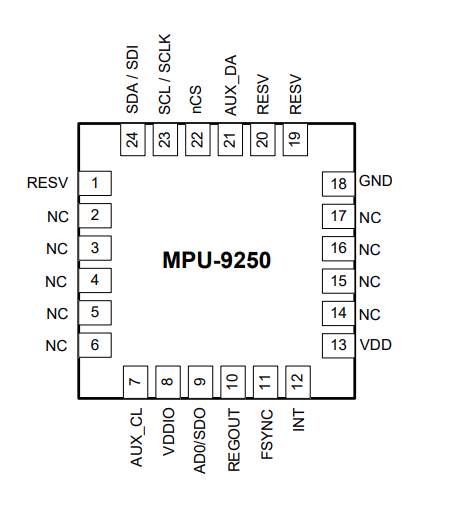
\includegraphics[scale=0.4]{images/mpu-9250-pinout.png}}
  \caption{Pin Out διάγραμμα του MPU-9250 (QFN packaging) \cite{evensense:20}}
  \label{fig:mpu-9250-qfn}
\end{figure}

\subsubsection{Ανάλυση καταλληλότητας}
O MPU-9250 είναι ένα προγραμματιζόμενο ψηφιακό κύκλωμα αισθητήρα επιτάχυνσης CMOS-MEMS. Έχει δηλαδή, ενσωματωμένους προγραμματιζόμενους καταχωρητές τους οποίους μπορούμε να προγραμματίσουμε μέσω Ι\textsuperscript{2}C (στα 400KHz) ή και SPI (στο 1MHz), παραμετροποιώντας έτσι τη λειτουργία του. Η κλίμακα των μετρήσεων επιτάχυνσης που επιτρέπει είναι \textpm 2g, \textpm 4g, \textpm 8g, \textpm 16g ανάλογα με την παραμετροποίηση που του έχουμε κάνει. Επίσης διαθέτει ενσωματωμένους ADC-converters με ανάλυση 16-bit για την ψηφιοποίηση των μετρήσεων. Έτσι συμπεραίνουμε ότι πληρεί τα κριτήρια που θέτουμε ως προς το εύρος και τη ποιότητα τον μετρήσεων. Οι συνιστώμενες συνθήκες λειτουργίας του είναι από \ang{-40} C εώς \ang{+85} C. Ο αισθητήρας παρέχει λειτουργικότητα self-test η οποία μπορεί να αποβεί πολύ χρήσιμη σε βελτιώσεις του συστήματος μας. Επίσης ο συγκεκριμένος αισθητήρας υποστηρίζει sleep-mode από το οποίο χρειάζεται 20ms για να επανέλθει, αυτός ο χρόνος είναι το 20\% του ενός κύκλου ABS (100ms) και επιλέγουμε να μην τον χρησιμοποιήσουμε. Ο αισθητήρας επίσης περιλαμβάνει ενσωματωμένο ένα προγραμματιζόμενο χαμηλοπερατό φίλτρο (LPF) για την μείωση του θορύβου στις υψηλές συχνότητες του σήματος δειγματοληψίας. Ακόμα περιλαμβάνει περαμετροποιήσιμο ρυθμό δεδομένων στο output (output data rate) το οποίο καθορίζεται από το ενεργειακό mode λειτουργίας του. Στο low-power mode αυτό έχει εύρος 0.24-500Hz και στο normal-mode έχει εύρος 4-4000Hz. Και στα 2 modes επιτρέπεται χρήση LPF, μόνο όμως στο normal έχουμε μεταβλητό bandwidth. Στο normal-mode, μας φάνηκε χρήσιμο το LPF παρότι δεν το συμπεριλάβαμε στον αρχικό σχεδιασμό, αφού δεν θέλουμε να επηρεαστεί ο αλγόριθμος μας από ατέλειες του οδοστρώματος αλλά και από άλλους πιθανούς θορύβους που περιέχει το σήμα μας. Ο αισθητήρας δεν ενδείκνυται για χρήση σε εφαρμογές της βιομηχανίας οχημάτων, καθώς δεν είναι συμβατός με τα πρότυπα αυτής για το συγκεκριμένο είδος συστατικών. Πιο συγκεκριμένα παρατηρούμε ότι δεν είναι συμβατός με το πρότυπο AEC-Q100. Ο συγκεκριμένος αισθητήρας προορίζεται ιδανικά για εφαρμογές χειριστηρίων και wearables. Τέλος, κόστος του συγκεκριμένου αισθητήρα την στιγμή που γράφεται αυτή η εργασία ανέρχεται περίπου στα 5\$ στη λιανική, το οποίο είναι λίγο περισσότερο από όσο περίπου θα επιθυμούσαμε, το οποίο είναι μη αποδεκτό αν σκεφτούμε πως κάνουμε και μικρή αξιοποίηση των δυνατοτήτων του.

\subsubsection{Προγραμματισμός αισθητήρα}
Ο παραμετροποίηση του συγκεκριμένου αισθητήρα γίνεται κυρίως μέσω τον καταχωρητών 28-31 τους οποίους μπορούμε να διαβάσουμε και να γράψουμε μέσω των πρωτοκόλλων. Ο καταχωρητής 28 επιτρέπει τη παραμετροποίηση του self-testing και της κλίμακας των μετρήσεων. Ο καταχωρητής 29 μας επιτρέπει την ενεργοποίηση/απ\-ενεργοποίηση του LPF καθώς και του bandwidth του. Οι καταχωρητές 30 και 31 είναι υπεύθυνοι για τη θέσπιση ορίου συχνότητας και επιτάχυνσης αντίστοιχα, από τα οποία ξυπνάει ο αισθητήρας από το sleep mode. Για περισσότερες λεπτομέρειες ο αναγνώστης μπορεί να ανατρέξει στο Register Map and Descriptions του MPU-9250 \cite{evensense1:20}.

\begin{figure}[H]
\makebox[\textwidth][c]{  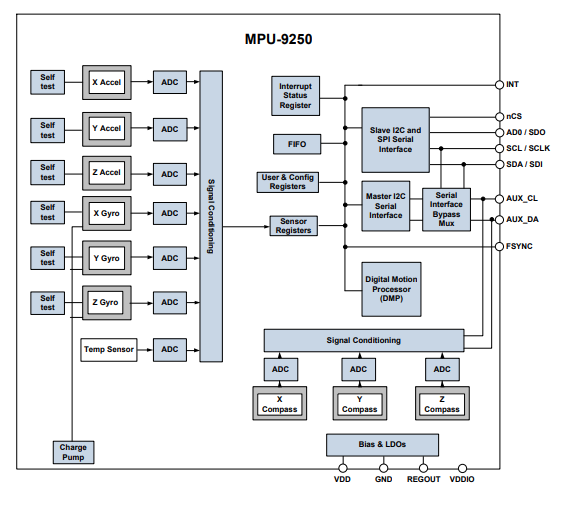
\includegraphics[scale=0.6]{images/mpu-9250-block-diagram.png}}
  \caption{Block διάγραμμα του MPU-9250 \cite{evensense:20}}
  \label{fig:mpu-9250-block-diagram}
\end{figure}

\subsubsection{Πείραμα και πειραματικές μετρήσεις}
Για τις πειραματικές μετρήσεις, χρησιμοποιήσαμε την παρακάτω συνδεσμολογία όπως φαίνεται στο Σχήμα \ref{fig:mpu-9250-implementation-schematic}. Χρησιμοποιήθηκε ένα developement board με το ESP32 και τον αισθητήρα συνδεδεμένο σε αυτό. Η σύνδεση του με τον μικροελεγκτή του ESP32 έγινε μέσω I\textsuperscript{2}C. Τo developement board συνδέθηκε μέσω UART-to-USB με τον φορητό υπολογιστή στον οποίο καταγράφτηκαν οι μετρήσεις, εκεί φιλτραρίστηκε η είσοδος και κρατήθηκε μόνο ο Χ άξονας και παρουσιάζονται στο Σχήμα \ref{fig:mpu-9250-implementation-samples-30-40} και στο Σχήμα \ref{fig:mpu-9250-implementation-samples-45} παρακάτω.
\par
Ο προγραμματισμός του αισθητήρα έγινε ως εξής για κάθε πειραματική μέτρηση. Όλες οι μετρήσεις είχανε κλίμακα μέτρησης \tpm 4g, το οποίο στον συγκεκριμένο αισθητήρα έχει ανάλυση 8 LSB/g \footnote{Αυτό σημαίνει ότι αν μεταβληθεί κατά 1g η επιτάχυνση τότε θα έχουμε μεταβολή των 8 LSB (λιγότερο σημαντικών ψηφίων)}. Αυτό περιορίζει τη χρήσιμη πληροφορία μας πρακτικά στα 12 bits από τα 16 bits που είναι θεωρητικά το μέγιστο και έχουμε θέσει ως απαίτηση. Όλες οι μετρήσεις είχανε LPF με bandwidth 42Hz και sample rate 200Hz, εκτός της τελευταίας που είχε LPF με bandwidth 5Hz και sample rate 30Hz. Παρατηρήσαμε ότι η χρήση 5Hz LPF βοηθάει στην εξομάλυνση των δεδομένων, ωστόσο αυξάνει ιδιαίτερα το χρόνο που χρειάζεται για να εξαχθεί η μέτρηση από τα 2ms στα 30ms περίπου. Αυτή η καθυστέρηση είναι μη αποδεκτή για το σύστημα μας αφού σπαταλά το 30\% ενός κύκλου ABS (100ms) ωστόσο. Από τα λίγα πειράματα που διεξήχθησαν, καταλήξαμε πως αυτός ο αισθητήρας παρότι είναι σχεδόν κατάλληλος για το σύστημα μας αφού ικανοποιεί τους περισσότερους σχεδιαστικούς περιορισμούς, μάλλον θα υπάρχουν περιθώρια βελτίωσης από κάποιον με γρηγορότερο τρόπο εξομάλυνσης.

\begin{figure}[H]
\makebox[\textwidth][c]{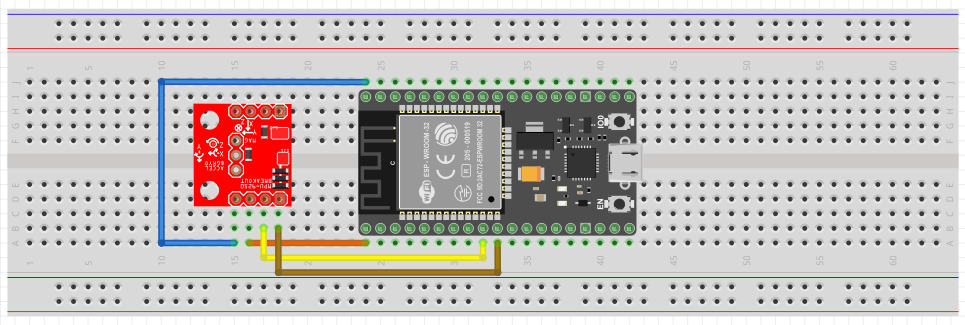
\includegraphics[scale=0.40]{images/mpu-9250-implementation-schematic.png}}
\caption{Διάγραμμα πειραματικής υλοποίησης, ESP32 developement board συνδεδεμένο με τον MPU-9250}
\label{fig:mpu-9250-implementation-schematic}
\end{figure}

\begin{figure}[H]
    \centering
    \subfigure{\textwidth}{
        \centering
        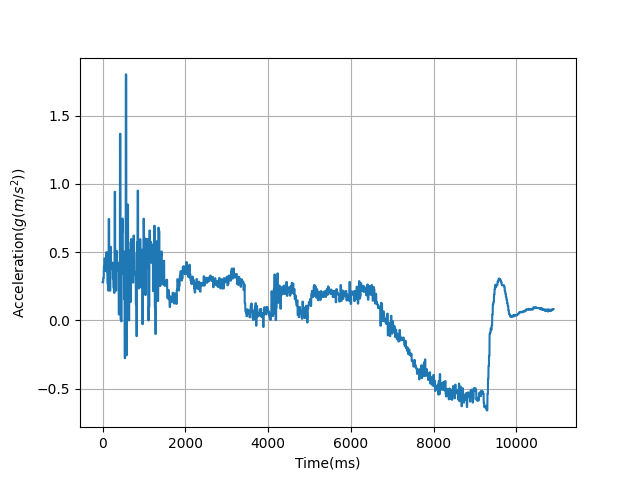
\includegraphics[width=0.49\textwidth]{images/samples_km30.txt.png}
        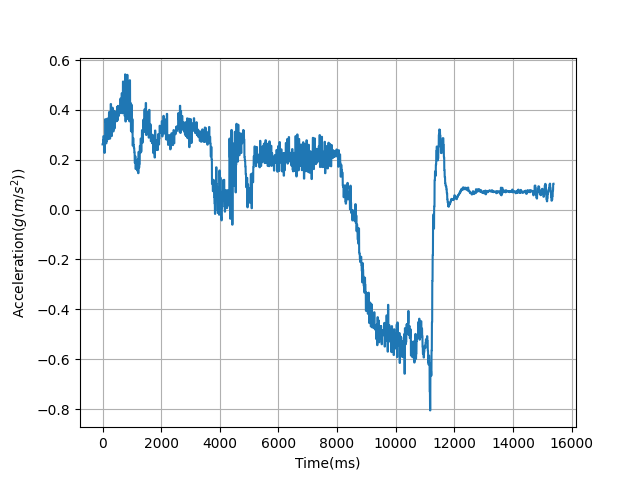
\includegraphics[width=0.49\textwidth]{images/samples_km40.txt.png}
        \caption{Πειραματικές μετρήσεις επιβράδυνσης/χρόνου απότομης πέδησης από τελική ταχύτητα 30 km/h με 42Hz LPF (αριστερά) και 40 km/h με 42Hz (δεξιά).}
        \label{fig:mpu-9250-implementation-samples-30-40}
    }
\end{figure}

\begin{figure}[H]
    \centering
    \subfigure{\textwidth}{
        \centering
        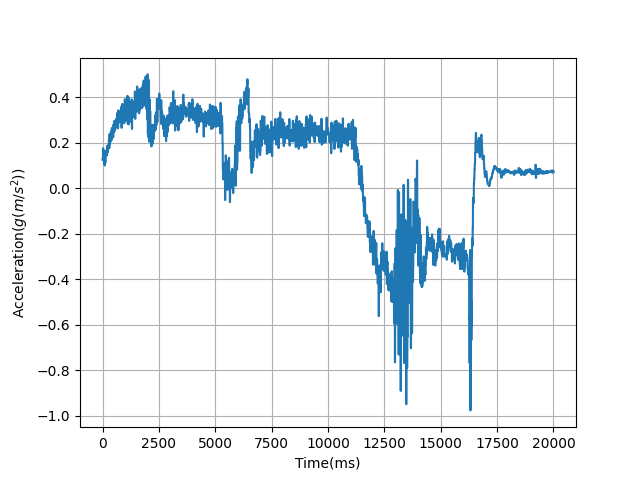
\includegraphics[width=0.49\textwidth]{images/samples_km45.txt.png}
        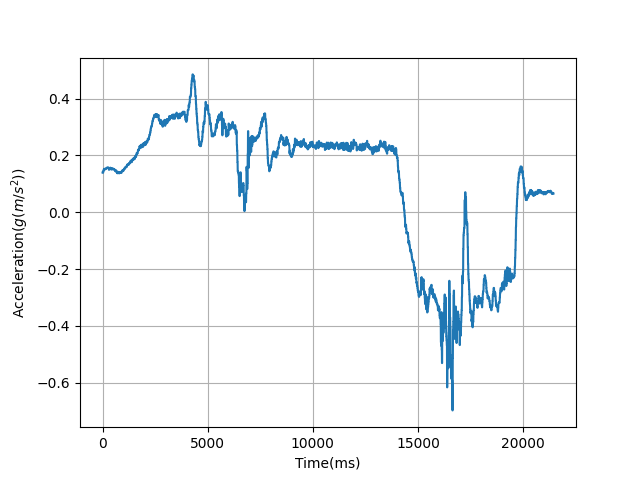
\includegraphics[width=0.49\textwidth]{images/samples_km45_hz5.txt.png}
        \caption{Πειραματικές μετρήσεις επιβράδυνσης/χρόνου απότομης πέδησης από τελική ταχύτητα 40 km/h με 42KHz LPF (αριστερά) και με 5KHz LPF (δεξιά)}
        \label{fig:mpu-9250-implementation-samples-45}
    }
\end{figure}

\section{Διαδικασίες ελέγχου ορθής λειτουργίας}
Επιλέγουμε να κάνουμε έλεγχο ορθής λειτουργίας μόνο του αισθητήρα ΜPU-9250 που χρησιμοποιήθηκε προηγουμένως. Το setup για την υλοποίηση παραμένει το ίδιο.

\subsection{MPU-9250}
Ο συγκεκριμένος αισθητήρας υποστηρίζει λειτουργία self-testing. Συνοπτικά το self-testing στον συγκεκριμένο αισθητήρα λειτουργεί ως εξής. Αρχικά η λειτουργία self-testing είναι απενεργοποιημένη. Τώρα έστω ότι σε ένα συγκεκριμένο άξονα (π.χ. στον Χ) η επιτάχυνση που του ασκείται είναι σταθερή και ίση με $a_x$. Όταν ενεργοποιούμε το self-testing με κάποιο ηλεκτρονικό τρόπο από το εσωτερικό του αισθητήρα μεταβάλλεται αυτή η επιτάχυνση κατά ένα μικρό ποσό $\Delta_x$ που το μετράει ο αισθητήρας ως $a_x + \Delta_x$, δηλαδή παράγεται μια πλαστή επιτάχυνση. Αν το $\Delta_x$ εμπίπτει εντός κάποιος ορίων που έχει θεσπίσει το εργοστάσιο (είναι αποθηκευμένα μέσα στον αισθητήρα) τότε ο αισθητήρας περνάει το test αλλιώς αποτυγχάνει.

\subsubsection{Προγραμματισμός αισθητήρα για self-test}
O προγραμματισμός του αισθητήρα για το self-test έγινε όπως περιγράφεται αναλυτικά στον οδηγό \cite{evensense2:20} του αισθητήρα που υπάρχει αποκλειστικά για αυτό το σκοπό. Συνοπτικά ο προγραμματισμός το έγινε ως εξής. Ο αισθητήρας πρέπει να είναι ακίνητος. Πρώτα ρυθμίζουμε την κλίμακα μέτρησης και τα φίλτρα του αισθητήρα σε κάποιες συγκεκριμένες τιμές. Στη συνέχεια παίρνουμε ένα συγκεκριμένο αριθμό δειγμάτων από τον άξονα Χ και τα αποθηκεύουμε στο ESP32. Έπειτα ενεργοποιούμε τη λειτουργία self-test μέσω του καταχωρητή 28. Επαναλαμβάνουμε τις μετρήσεις και τις αποθηκεύουμε. Σταματάμε τη self-test λειτουργία. Υπολογίζουμε τη μέση απόκλιση. Διαβάζουμε τα εργοστασιακά όρια που είναι αποθηκευμένα στον αισθητήρα και τα συγκρίνουμε με αυτά που υπολογίσαμε και αποφασίζουμε για την επιτυχία της δοκιμής.

\subsubsection{Πειραματικές μετρήσεις self-test}
Στις Εξόδους προγράμματος \ref{code1} και \ref{code2} φαίνονται τα αποτελέσματα των πειραματικών μετρήσεων. Στην Έξοδο προγράμματος \ref{code1} φαίνεται ο αισθητήρας αποτυγχάνει το test γιατί ήταν είχε μεταβαλλόμενη επιτάχυνση εκείνη τη στιγμή επειδή τον κινούσαμε με το χέρι μας. Στην Έξοδο προγράμματος \ref{code2} αριστερά ο αισθητήρας είναι ακίνητος και επιτυγχάνει το test.

\begin{lstlisting}[frame=single,caption=Αποτυχημένο self-test για τον Y άξονα,label=code1]
regularBias: +7835 | regularBiasGravity: +0.48
selfTestBias: +8941 | selfTestBiasGravity: +0.55
shiftCode: +99 
shiftProduction: +0.42
shiftResponse: +0.07
shiftVariation: -0.84
Accel self-test: [Y=FAIL]
\end{lstlisting}

\begin{lstlisting}[frame=single,caption=Επιτυχημένο self-test για τον X άξονα,label=code2]
regularBias: +137 | regularBiasGravity: +0.01
selfTestBias: +7297 | selfTestBiasGravity: +0.45
shiftCode: +101
shiftProduction: +0.43
shiftResponse: +0.44
shiftVariation: +0.01
Accel self-test: [X=OK]
\end{lstlisting}

\section{Βελτιστοποιήσεις και προτάσεις}

Μια πιθανή προσθήκη για τη βελτίωση της ασφάλειας του συστήματος και των χρηστών του θα ήταν η υποστήριξη ενδείξεων κακής λειτουργίας ή φθοράς μερών του συστήματος. Έχουμε να κάνουμε με ένα σύστημα από το οποίο εξαρτώνται βασικές λειτουργίες του αυτοκινήτου. Για παράδειγμα, θα ήταν πολύ επικίνδυνο αν το όχημα ανέπτυσσε ταχύτητα και έπρεπε να φρενάρει ενώ δεν δουλεύουν οι βαλβίδες ή η αντλία ή αν έχει χαλάσει οποιοδήποτε μέρος του συστήματος γενικότερα. Θα μπορούσαμε εν μέρη να λύσουμε αυτό το πρόβλημα εισάγοντας σε επίπεδο λογισμικού ή υλικού έναν έλεγχο για όλα τα υποσυστήματα ότι λειτουργούν σωστά από την ECU, ο οποίος θα εκτελούνταν κάθε φορά που έπαιρνε εμπρός το αμάξι και ίσως ανά τακτά χρονικά διαστήματα κατά τη διάρκεια λειτουργίας του. Αυτό ωστόσο ίσως να απαιτούσε και την επέκταση του απλού πρωτοκόλλου επικοινωνίας που έχουμε ορίσει ώστε να μπορούν οι επιμέρους μικροελεγκτές κάθε συστήματος να ενημερώνονται για των ελέγχων από την ECU και στην συνέχεια να μπορούν να επιστρέφουν κατάλληλα μηνύματα σφαλμάτων. Η ECU με τη σειρά της θα πρέπει να επικοινωνεί με κάποια κεντρική ECU και να την ενημερώνει για περίπτωση σφάλματος ή να υποστηρίζει πρότυπα διάγνωσης σφαλμάτων όπως το OBD και OBD-II τα οποία ενεργούν επί του ήδη υπάρχοντα διαύλου CAN.

Μια ακόμα πιθανή βελτίωση θα ήταν η χρήση ξεχωριστού διαύλου μόνο για την επικοινωνία μεταξύ της ABS ECU και των αισθητήρων, μιλάμε για την περίπτωση του PSI-5 που αναφέρθηκε νωρίτερα. Αυτή η προσθήκη θα προκαλούσε αισθητή βελτίωση στη περίπτωση οχημάτων με υπερφορτωμένο δίαυλο CAN. Στην θεωρητική ανάλυση του διαύλου επικοινωνίας είχαμε υποθέσει λόγω της φύσης του συστήματος μας ότι αυτό έχει την μέγιστη προτεραιότητα επικοινωνίας και "κερδίζει πάντα" στον ανταγωνισμό για τη πρόσβαση στο δίαυλο και άρα δεν μας επηρεάζει πόσο υπερφορτωμένος είναι αυτός. Αυτό διευκόλυνε την ανάλυση μας ωστόσο στις μέρες μας ίσως να μην είναι και ιδιαίτερα ρεαλιστική υπόθεση καθώς σήμερα σε ένα όχημα σήμερα υπάρχουν αρκετά συστήματα τα οποία καλούνται να συνυπάρξουν με το ABS. Η προσθήκη ενός νέου διαύλου σίγουρα δε μειώνει το κόστος, πόσο μάλλον όταν το πρότυπο του δεν είναι ακόμα ευρέως διαδεδομένο στην αγορά. Ωστόσο λόγω της εξειδικευμένης χρήσης του πρωτοκόλλου αυτού δεν χρειαζόμαστε γενικού σκοπού μικροεπεξεργαστές και σύνθετα υποσυστήματα επικοινωνίας, όπως στον δίαυλο CAN. Το πρωτόκολλο επικοινωνίας είναι αρκετά απλό, πιο απλό από το CAN, και τα υποσυστήματα επικοινωνίας (π.χ. ελεγκτής διαύλου, πομποδέκτης στη περίπτωση του CAN) έρχονται ενσωματωμένα στα ολοκληρωμένα των αισθητήρων και αυτό εξισορροπεί κάπως την αύξηση του κόστους.

\section{Εργαλεία που χρησιμοποιήθηκαν}
Κατά την εκπόνηση της εργασίας χρησιμοποιήθηκαν τα παρακάτω εργαλεία και πλατφόρμες :
\begin{itemize}
\item DrawIO, Fritzing για rapid prototyping
\item Matplotlib για τα γραφήματα
\item \href{https://docs.espressif.com/projects/esp-idf/en/latest/esp32/} ESP-IoT Developement Framework (IDF), το οποίο είναι port του FreeRTOS για τη πλατφόρμα ESP32 με επιπλέον προσθήκες
\item Βιβλιοθήκη \href{https://github.com/natanaeljr/esp32-MPU-driver} για την διευκόλυνση των πειραματικών μετρήσεων του MPU-9250 στο ESP32
\end{itemize}

\newpage

\bibliographystyle{IEEEtran}
\bibliography{main}

\end{document}
